\chapter{Appendix Figures}

\begin{quote}
  \emph{Hold on. You have to slow down. You're losing it. You have to take a breath. Listen to yourself. You're connecting a computer bug I had with a computer bug you might have had and some religious hogwash. You want to find the number 216 in the world, you will be able to find it everywhere. 216 steps from a mere street corner to your front door. 216 seconds you spend riding on the elevator. When your mind becomes obsessed with anything, you will filter everything else out and find that thing everywhere.}
  
  \begin{flushright}
    —\smallcaps{Sol Robeson}, \emph{Pi}
  \end{flushright}
\end{quote}

\vspace{1em}

\begin{quote}
  \emph{Calm down, Doctor! Now's not the time for fear. That comes later.}
  
  \begin{flushright}
    —\smallcaps{Bane}, \emph{The Dark Knight Rises}
  \end{flushright}
\end{quote}

% For this appendix, undo tufte-latex's big margin
\newgeometry{left=1in,right=1in,bottom=1.5in,textwidth=6.5in,marginparsep=0pc,marginparwidth=0pc}
% Recalculate fancy header/footer after geometry change (otherwise page numbers are misplaced)
\fancyhfoffset[E,O]{0pt}

%%%%%
%
% MetaHybridLouvain Example
%
%%%%%

\begin{figure*}[p]
  \centering
  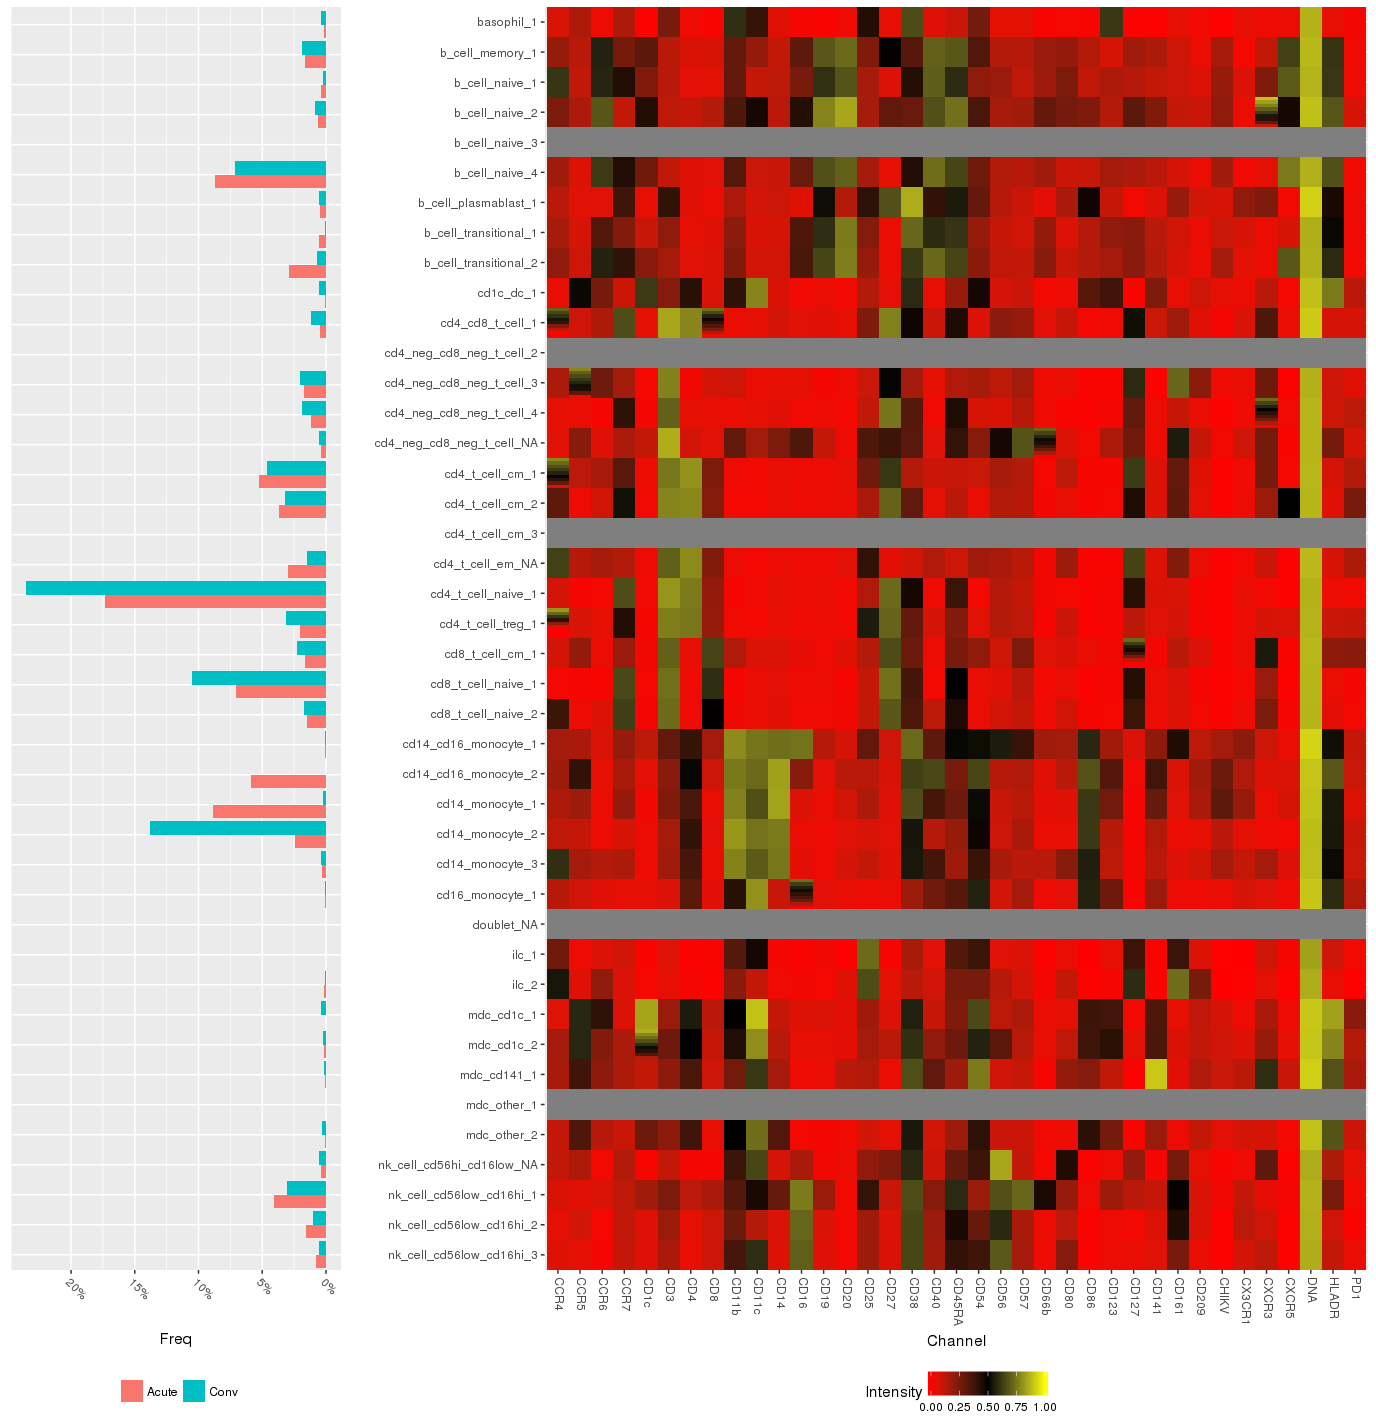
\includegraphics[width=\textwidth]{chap6/fig_S1a_MHL_example_1800}
  \fullwidthlabelcaption{fig:mhl_example}{Example output of \texttt{MetaHybridLouvain} for a representative paired CyTOF sample}{
  \textbf{Example output of \texttt{MetaHybridLouvain}} for the representative sample used in Figure \ref{fig:nodlabel_diag}, Figure \ref{fig:mhl_visne}, and \ref{fig:chikv_visne}. At left, frequencies for each sub-community at each timepoint, and at right, mini-heatmaps of channel values for each sub-community (plotted within each row). As expected, sub-communities generally show similar values among all channels for their constituent events, with some exceptions (vertical gradients within mini-heatmaps). \emph{Continued in Figure \ref{fig:mhl_example_cont}.}
  }
\end{figure*}

\begin{figure*}[p]
  \centering
  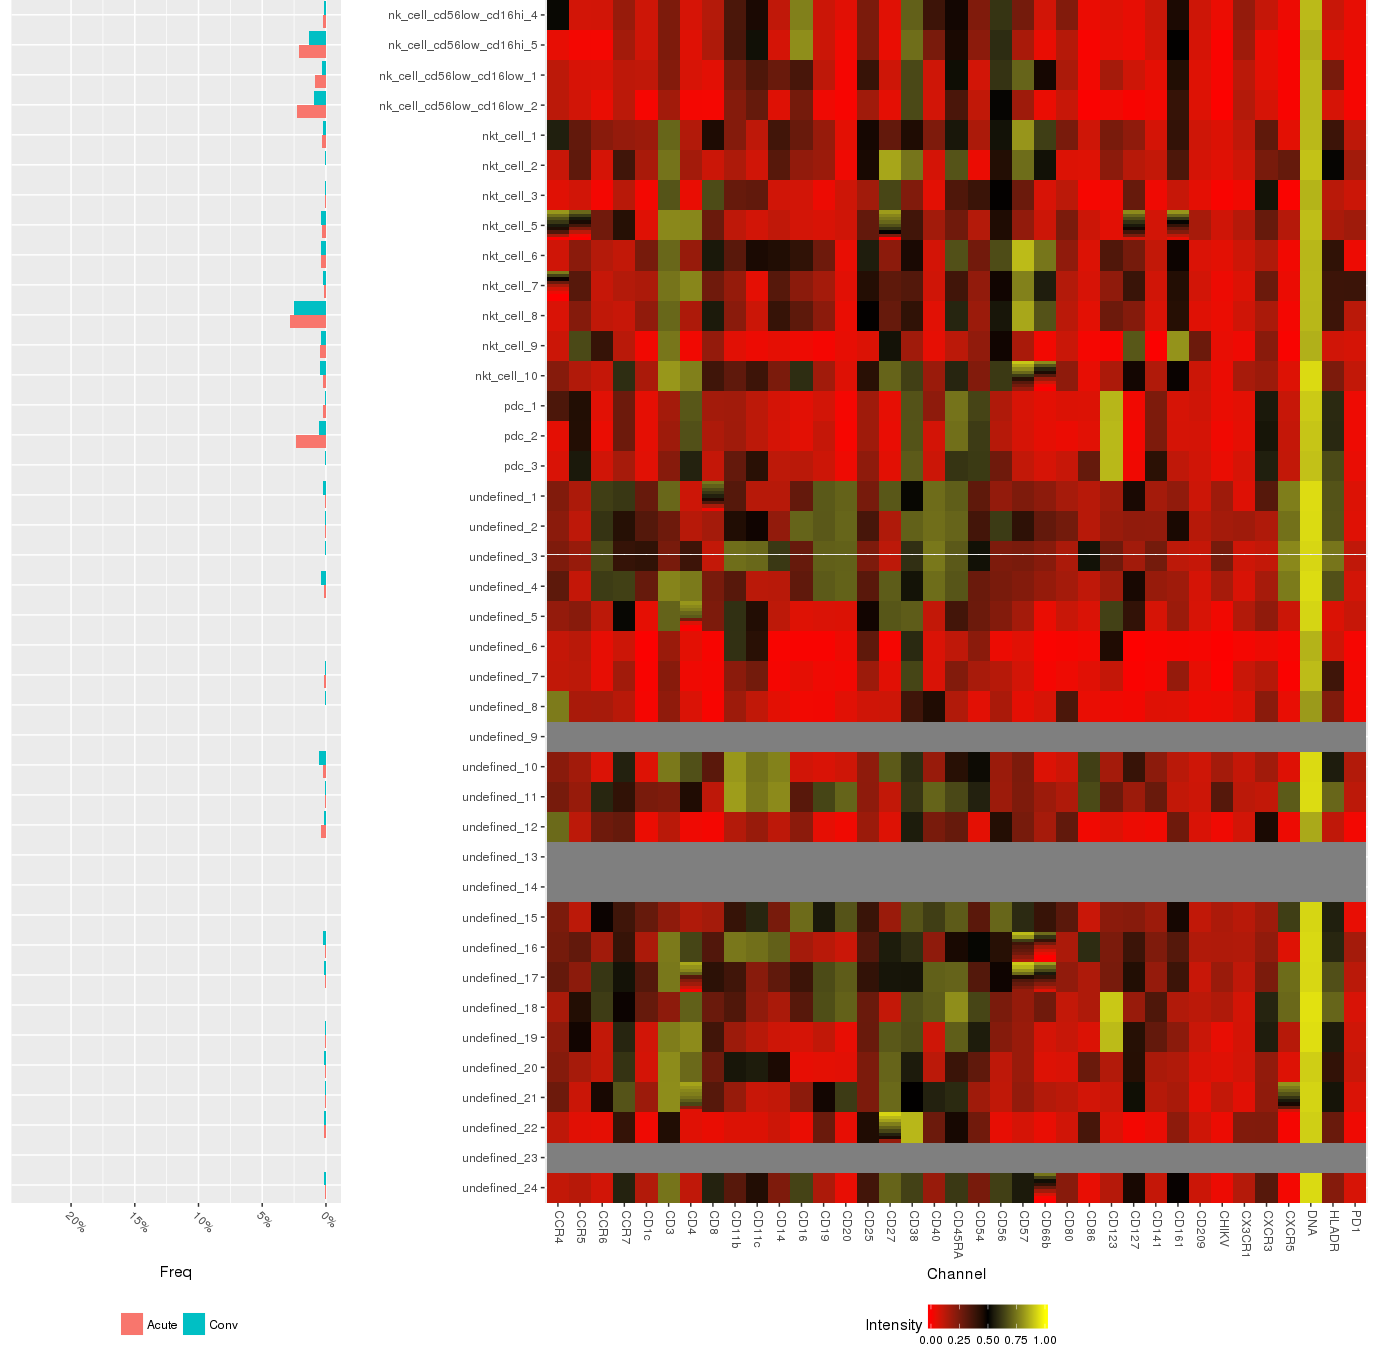
\includegraphics[width=\textwidth]{chap6/fig_S1b_MHL_example_1800}
  \fullwidthlabelcaption{fig:mhl_example_cont}{Example output of \texttt{MetaHybridLouvain} for a representative paired CyTOF sample, continued}{
  \textbf{Continuation of example output of \texttt{MetaHybridLouvain}} for the representative sample used in Figure \ref{fig:nodlabel_diag}, Figure \ref{fig:mhl_visne}, and \ref{fig:chikv_visne}. At left, frequencies for each sub-community at each timepoint, and at right, mini-heatmaps of channel values for each sub-community (plotted within each row). As expected, sub-communities generally show similar values among all channels for their constituent events, with some exceptions (vertical gradients within mini-heatmaps). \emph{Continued from Figure \ref{fig:mhl_example}.}
  }
\end{figure*}

%%%%%
%
% CD14CD16 Monocyte Sub-Community Differences
%
%%%%%

\begin{figure*}[p]
  \centering
  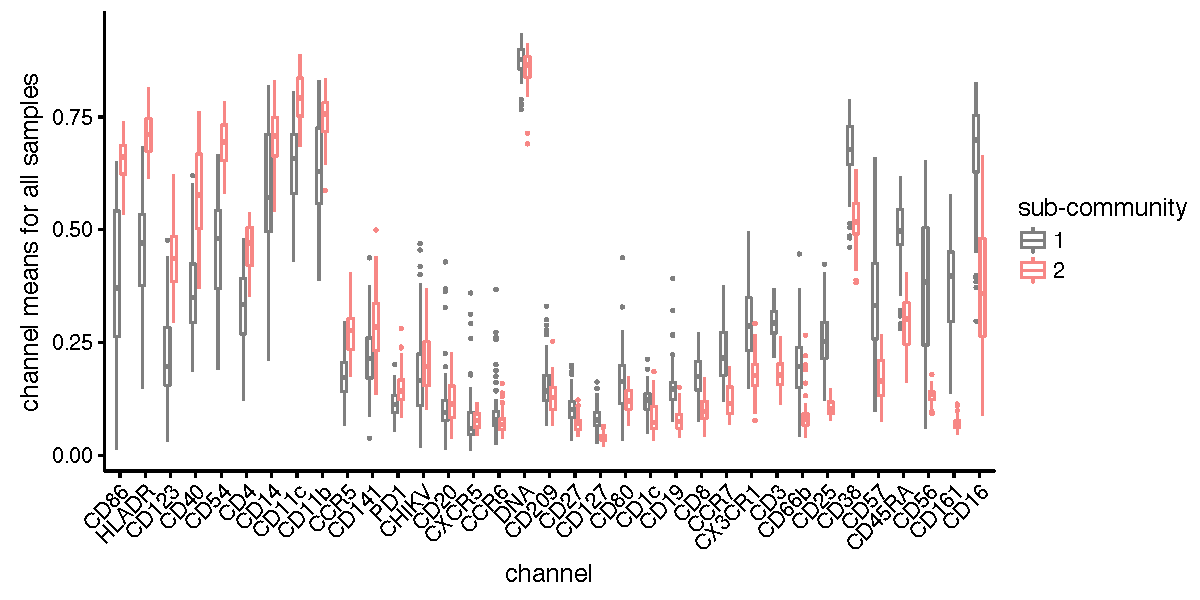
\includegraphics[width=\textwidth]{chap6/fig_S3_cd14cd16_monocytes_subpop_differences}
  \fullwidthlabelcaption{fig:cd14cd16_channel_diffs}{Differences in per-sample channel means between two CD14\sups{+}CD16\sups{+} sub-communities identified by \texttt{MetaHybridLouvain}}{
  \textbf{Differences in per-sample channel means between two CD14\sups{+}CD16\sups{+} sub-communities identified by \texttt{MetaHybridLouvain}.} 1 corresponds with the “intermediate” CD14\sups{++}CD16\sups{+} phenotype, while 2 corresponds with the “nonclassical” CD14\sups{+}CD16\sups{++} phenotype. The X axis is filtered to only the channels with differences significant at FDR < 0.05, and ordered from differences where sub-community 1 < 2 on the left to sub-community 1 > 2 on the right.
  }
\end{figure*}

\begin{figure*}[p]
  \centering
  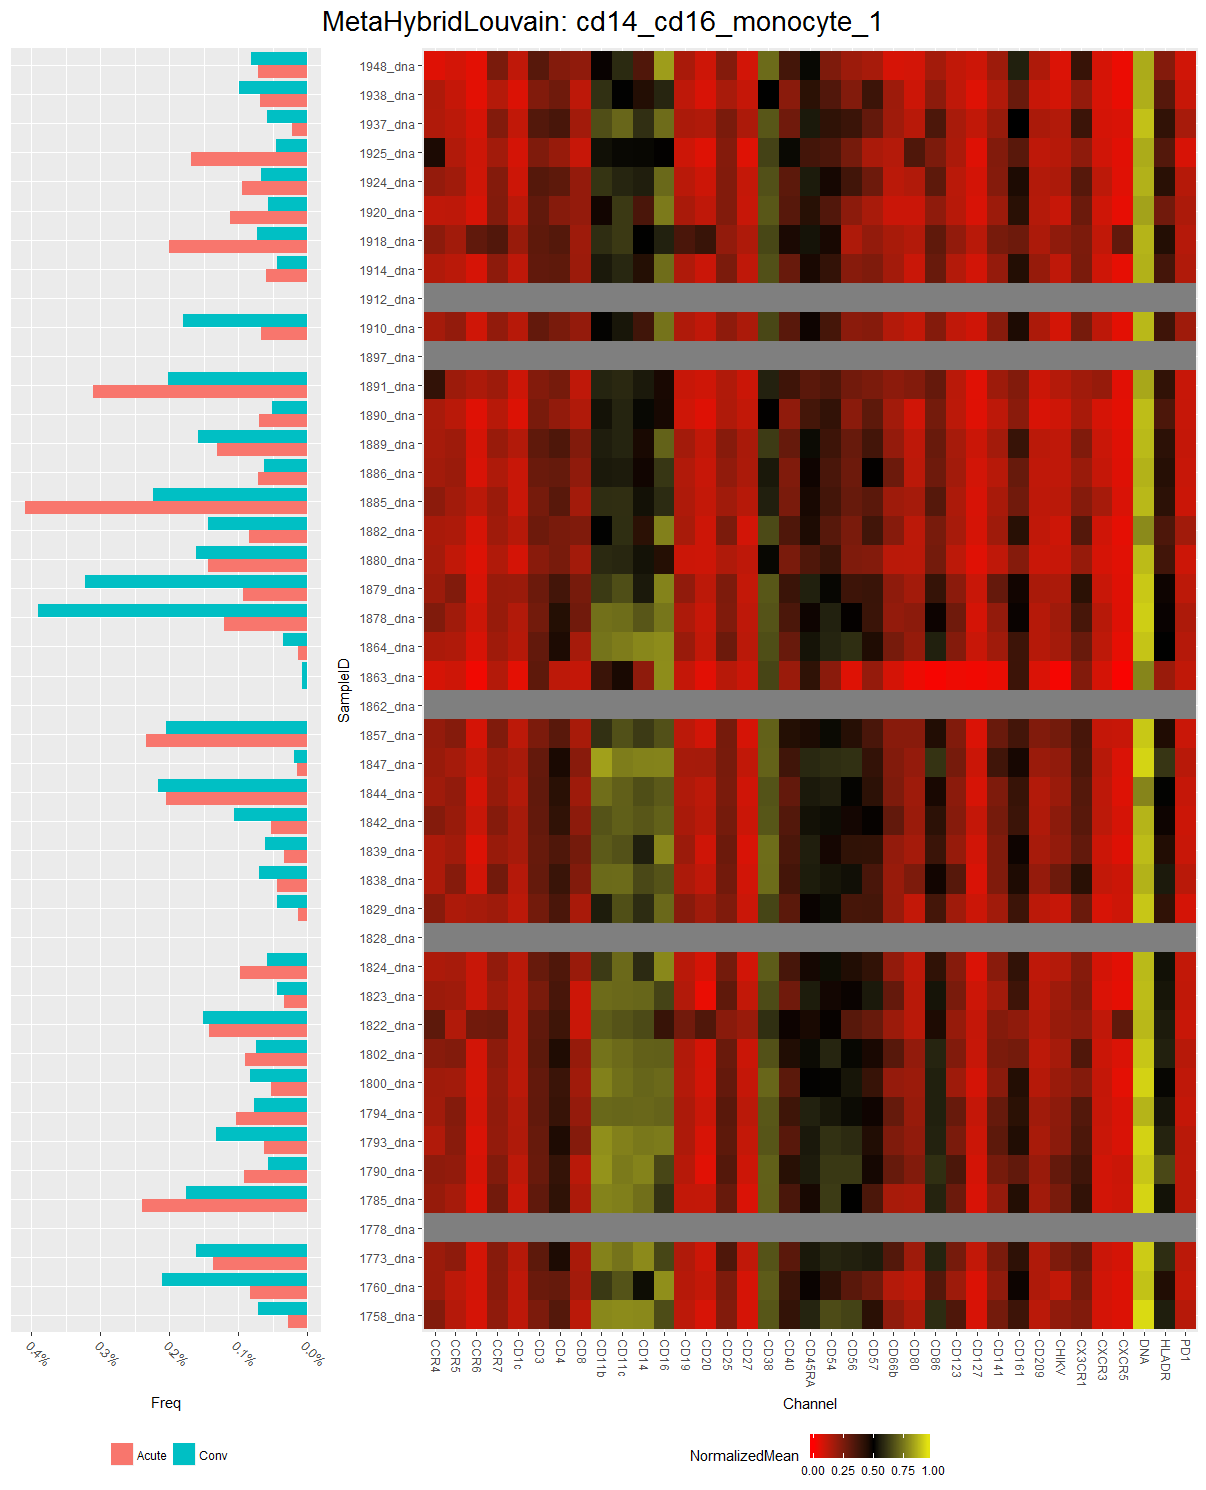
\includegraphics[width=0.9\textwidth]{chap6/fig_S4_cd14_cd16_monocyte_1}
  \fullwidthlabelcaption{fig:cd14cd16_subcomm_1_heatmap}{Summary of frequencies (per timepoint) and mean channel values for sub-community 1 of CD14\sups{+}CD16\sups{+} monocytes}{
  \textbf{Summary of frequencies (per timepoint) and mean channel values for sub-community 1 of CD14\sups{+}CD16\sups{+} monocytes}, across all samples. At left, frequencies in each sample split by timepoint; at right, mini-heatmaps of channel values for all events within this sub-community for each sample (plotted within each row). A gray row indicates this sub-community was not identified in this sample.
  }
\end{figure*}

\begin{figure*}[p]
  \centering
  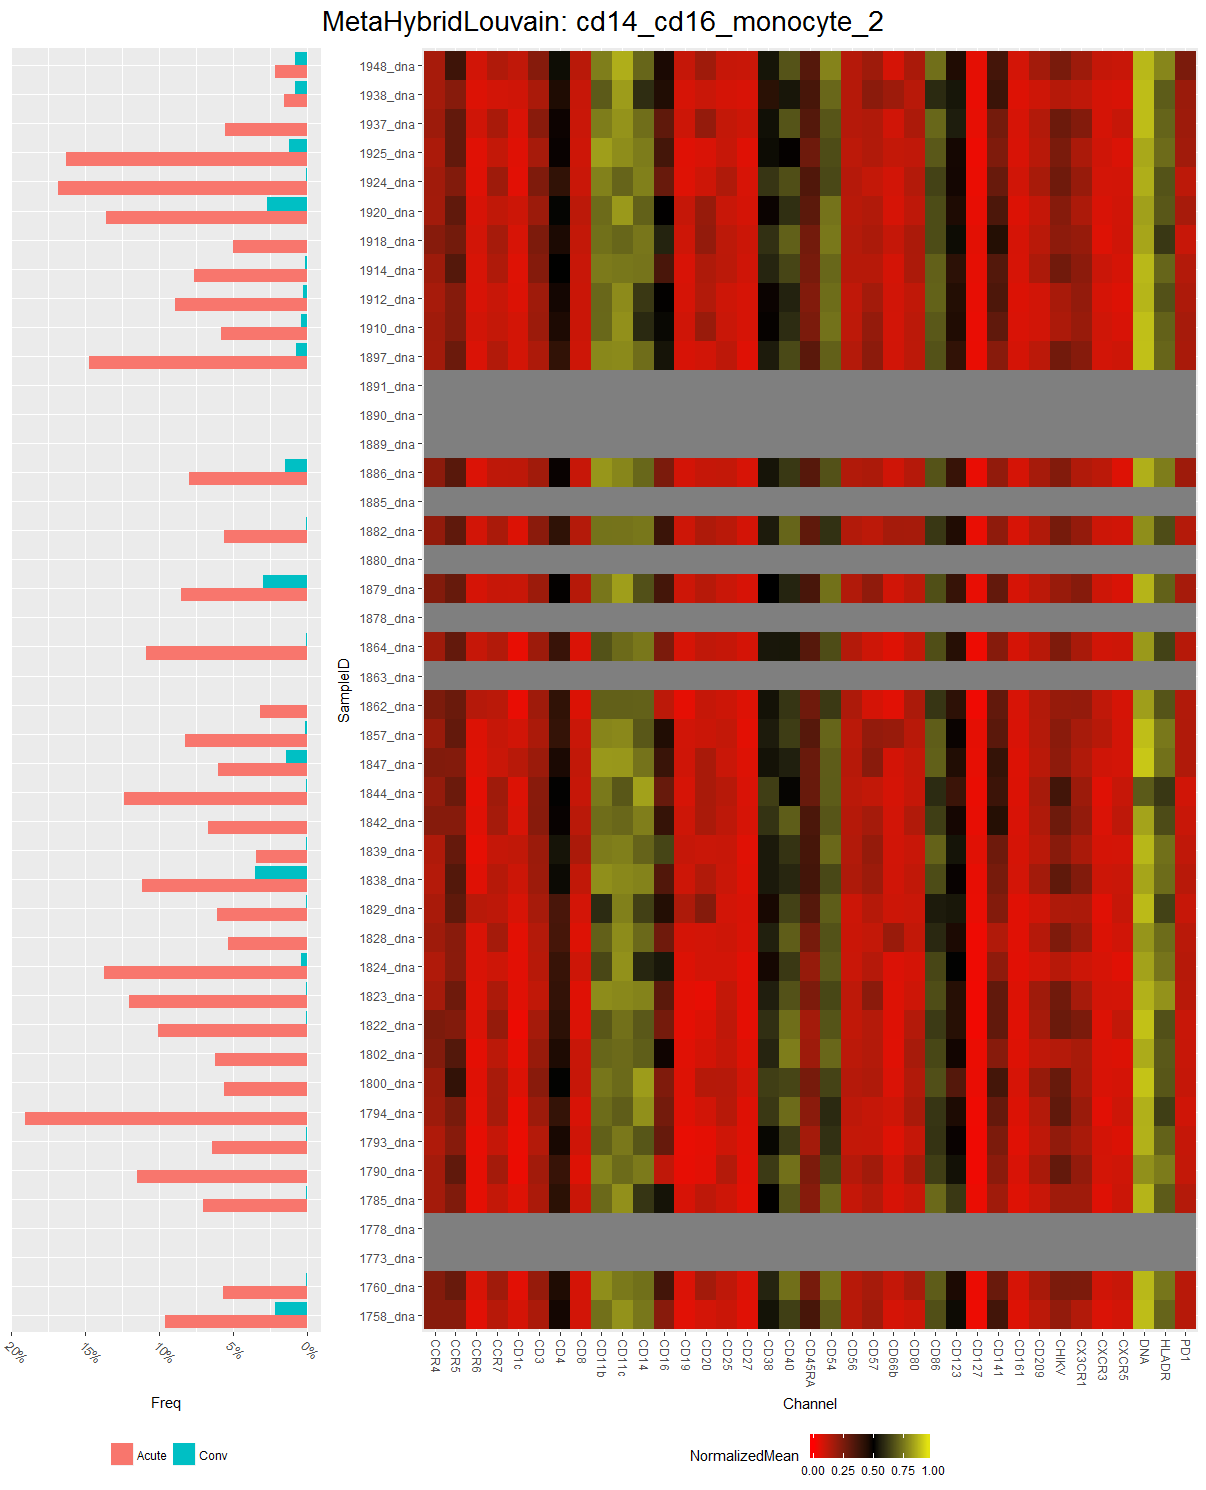
\includegraphics[width=0.9\textwidth]{chap6/fig_S5_cd14_cd16_monocyte_2}
  \fullwidthlabelcaption{fig:cd14cd16_subcomm_2_heatmap}{Summary of frequencies (per timepoint) and mean channel values for sub-community 2 of CD14\sups{+}CD16\sups{+} monocytes}{
  \textbf{Summary of frequencies (per timepoint) and mean channel values for sub-community 2 of CD14\sups{+}CD16\sups{+} monocytes}, across all samples. At left, frequencies in each sample split by timepoint; at right, mini-heatmaps of channel values for all events within this sub-community for each sample (plotted within each row). A gray row indicates this sub-community was not identified in this sample.
  }
\end{figure*}

%%%%%
%
% CD14 Monocyte Sub-Community Differences
%
%%%%%

\begin{figure*}[p]
  \centering
  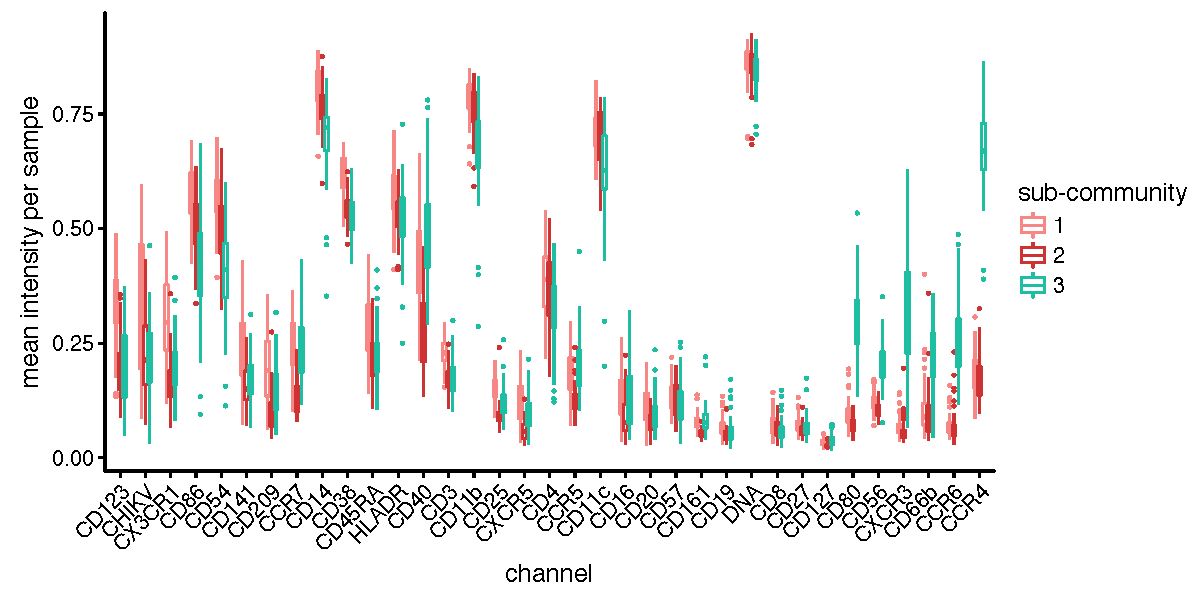
\includegraphics[width=\textwidth]{chap6/fig_S6_cd14_monocytes_subpop_differences}
  \fullwidthlabelcaption{fig:cd14_channel_diffs}{Differences in per-sample channel means between three CD14\sups{+} sub-communities identified by \texttt{MetaHybridLouvain}}{
  \textbf{Differences in per-sample channel means between three CD14\sups{+} sub-communities identified by \texttt{MetaHybridLouvain}.} The X axis is filtered to only the channels with differences significant at FDR < 0.05 (Kruskal-Wallis test), and ordered from differences where sub-community 1 is greater than the other two sub-communities on the left to differences where sub-community 1 is lower than the other two sub-communities on the right. 
  }
\end{figure*}

\begin{figure*}[p]
  \centering
  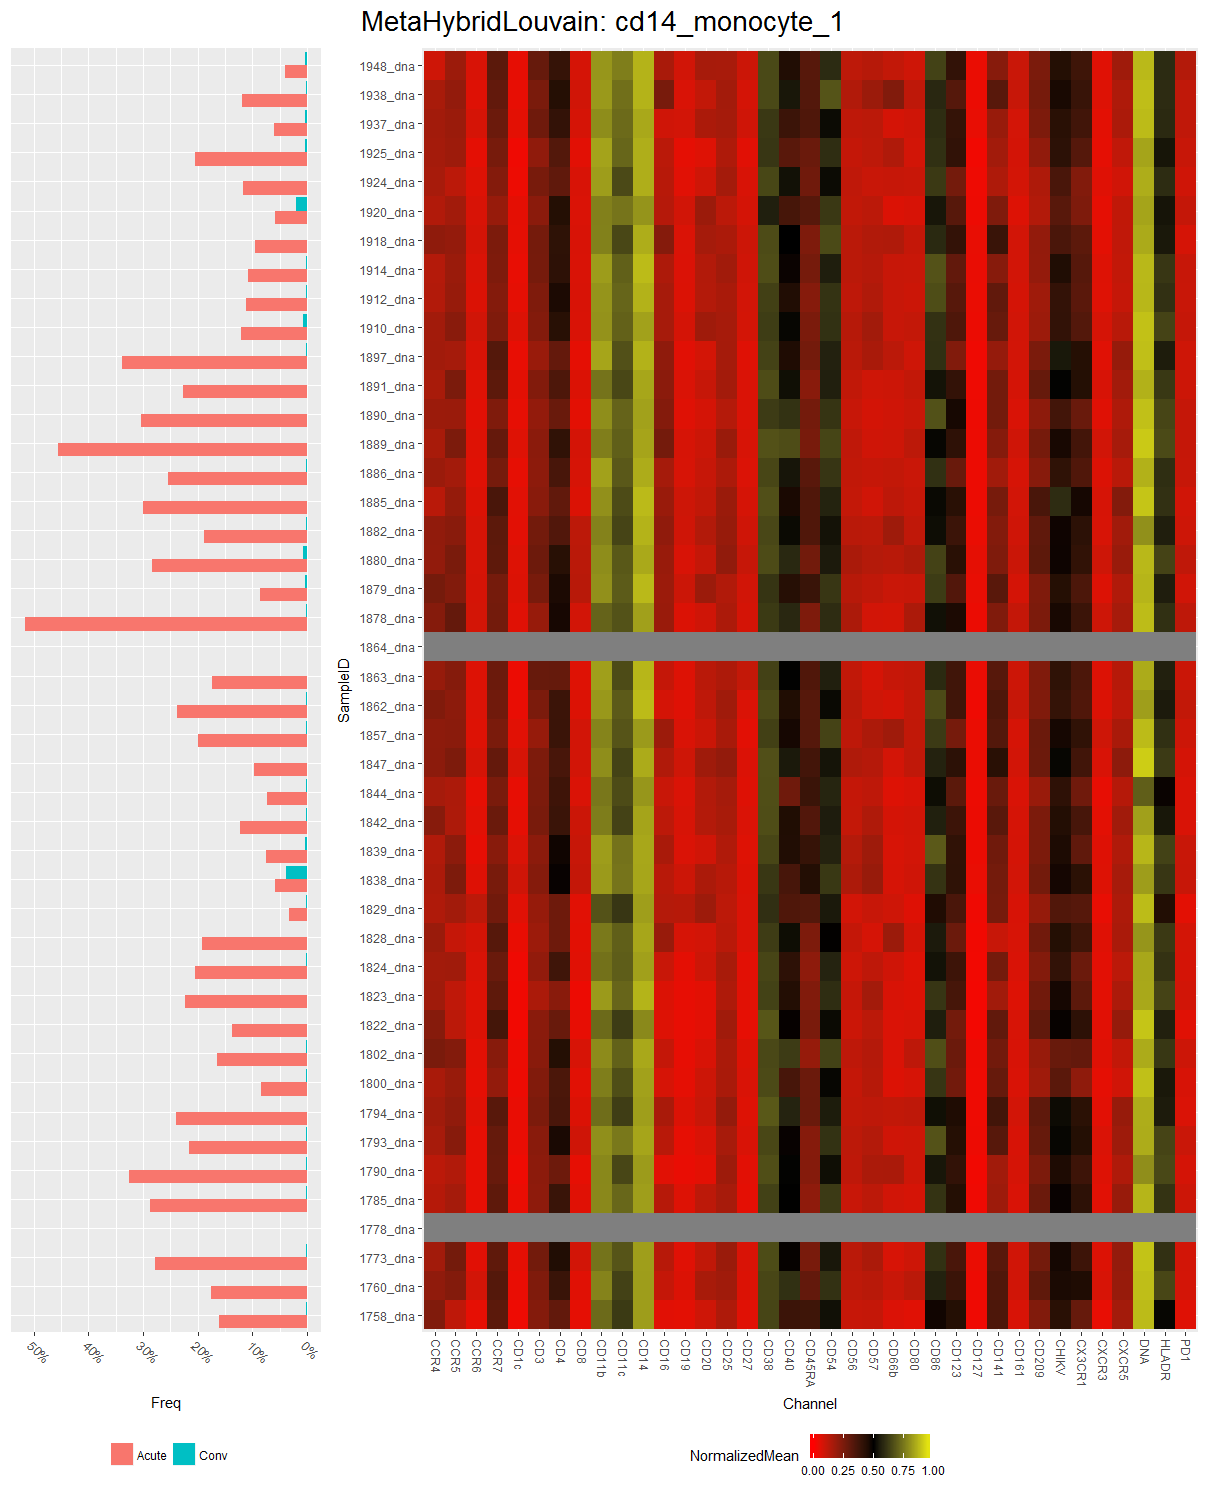
\includegraphics[width=0.9\textwidth]{chap6/fig_S7_cd14_monocyte_1}
  \fullwidthlabelcaption{fig:cd14_subcomm_1_heatmap}{Summary of frequencies (per timepoint) and mean channel values for sub-community 1 of CD14\sups{+} monocytes}{
  \textbf{Summary of frequencies (per timepoint) and mean channel values for sub-community 1 of CD14\sups{+} monocytes}, across all samples. At left, frequencies in each sample split by timepoint; at right, mini-heatmaps of channel values for all events within this sub-community for each sample (plotted within each row). A gray row indicates this sub-community was not identified in this sample.
  }
\end{figure*}

\begin{figure*}[p]
  \centering
  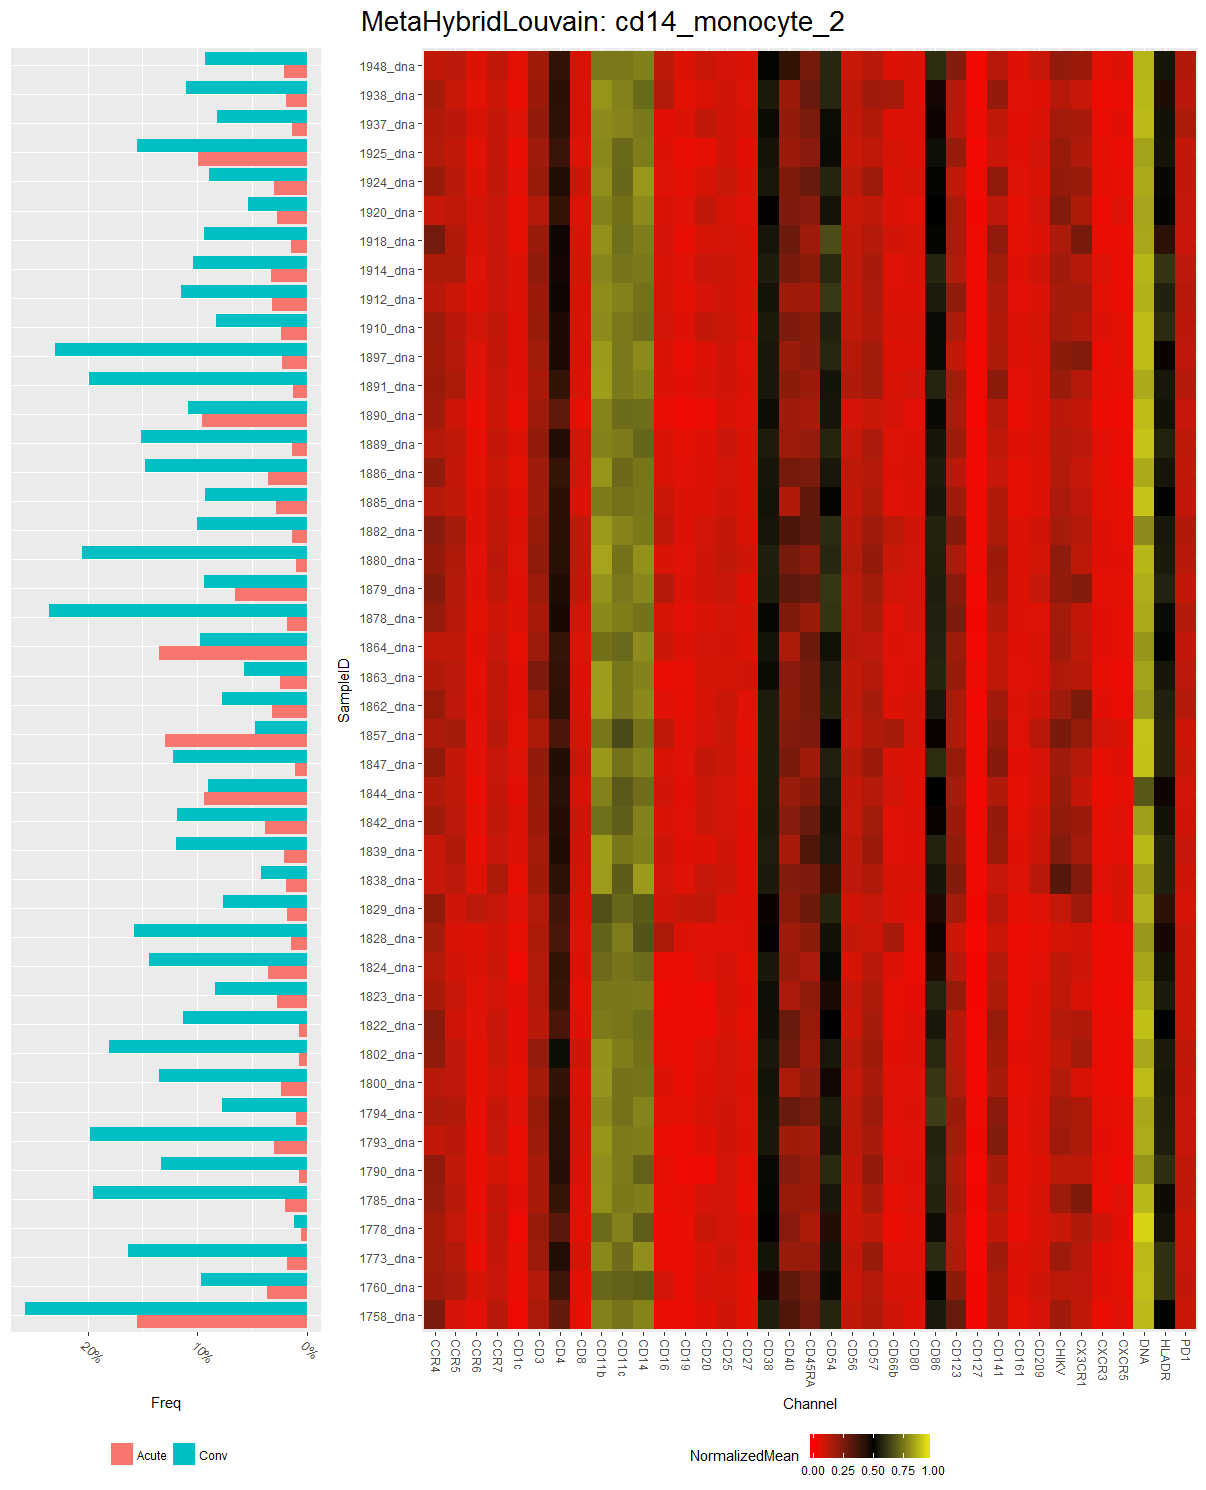
\includegraphics[width=0.9\textwidth]{chap6/fig_S8_cd14_monocyte_2}
  \fullwidthlabelcaption{fig:cd14_subcomm_2_heatmap}{Summary of frequencies (per timepoint) and mean channel values for sub-community 2 of CD14\sups{+} monocytes}{
  \textbf{Summary of frequencies (per timepoint) and mean channel values for sub-community 2 of CD14\sups{+} monocytes}, across all samples. At left, frequencies in each sample split by timepoint; at right, mini-heatmaps of channel values for all events within this sub-community for each sample (plotted within each row). A gray row indicates this sub-community was not identified in this sample.
  }
\end{figure*}

\begin{figure*}[p]
  \centering
  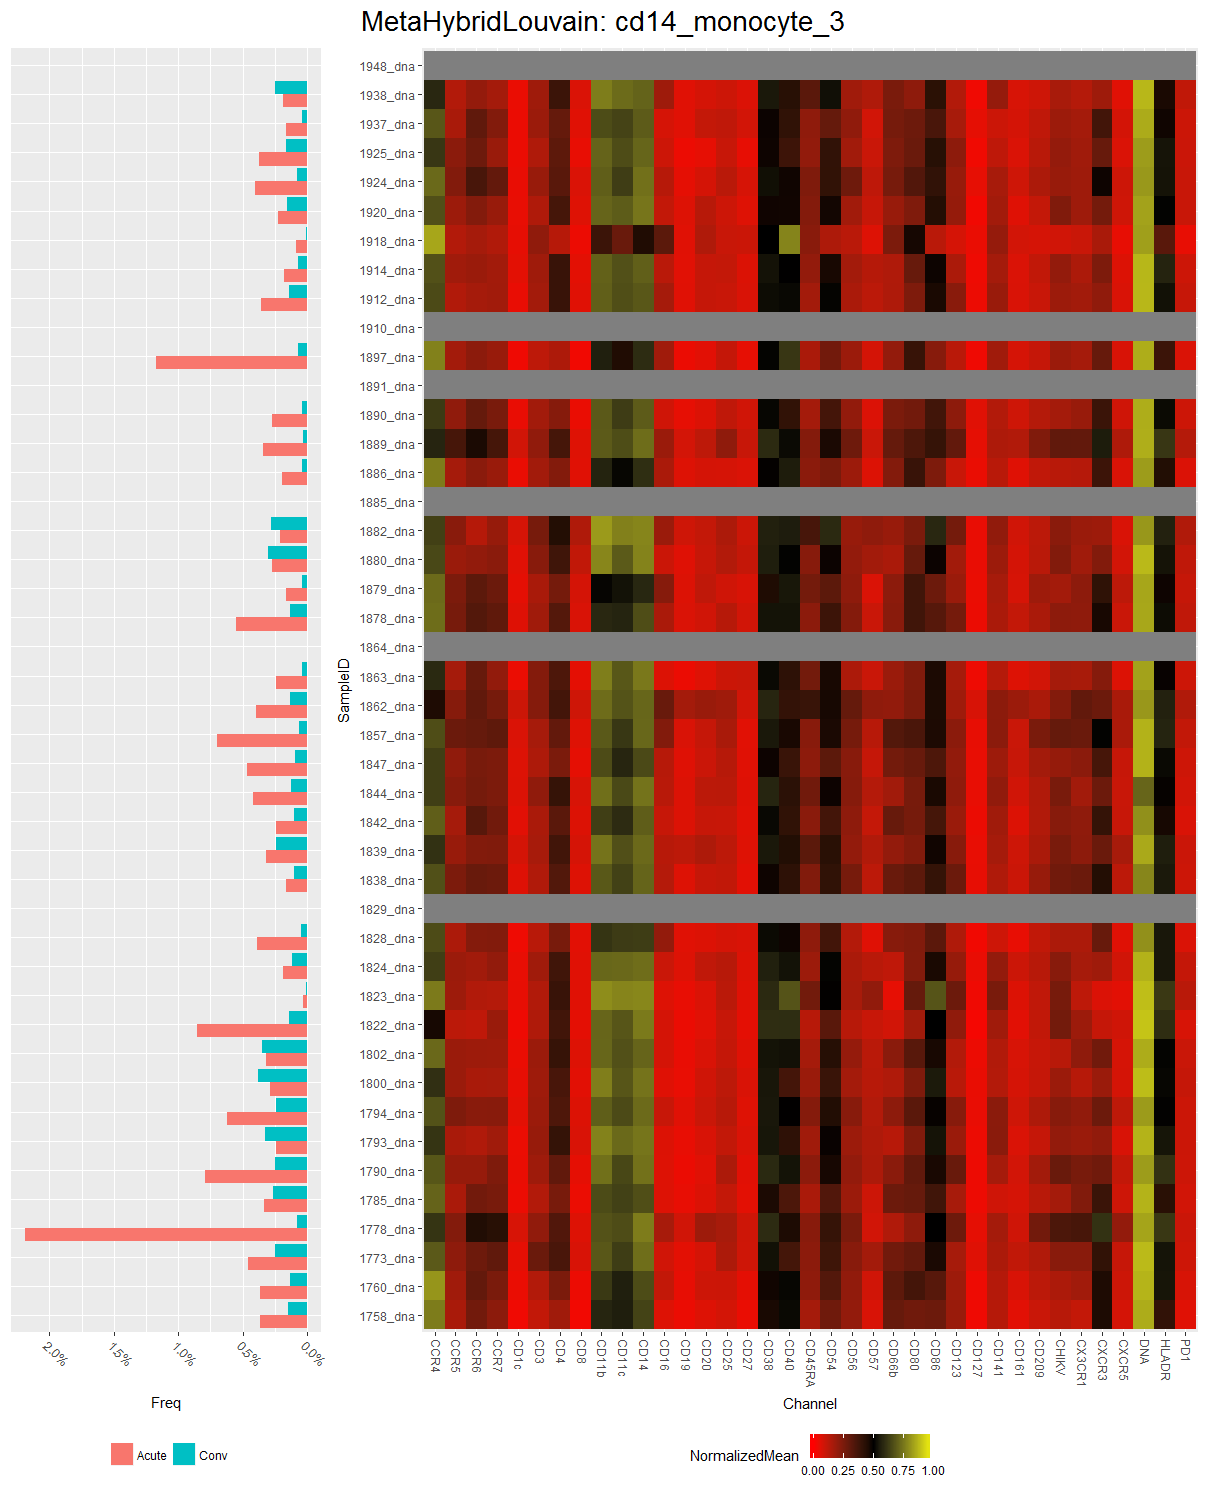
\includegraphics[width=0.9\textwidth]{chap6/fig_S9_cd14_monocyte_3}
  \fullwidthlabelcaption{fig:cd14_subcomm_3_heatmap}{Summary of frequencies (per timepoint) and mean channel values for sub-community 3 of CD14\sups{+} monocytes}{
  \textbf{Summary of frequencies (per timepoint) and mean channel values for sub-community 3 of CD14\sups{+} monocytes}, across all samples. At left, frequencies in each sample split by timepoint; at right, mini-heatmaps of channel values for all events within this sub-community for each sample (plotted within each row). A gray row indicates this sub-community was not identified in this sample.
  }
\end{figure*}

%%%%%
%
% Luminex and corrplots with CyTOF/mRNA
%
%%%%%

\begin{figure*}[p]
  \centering
  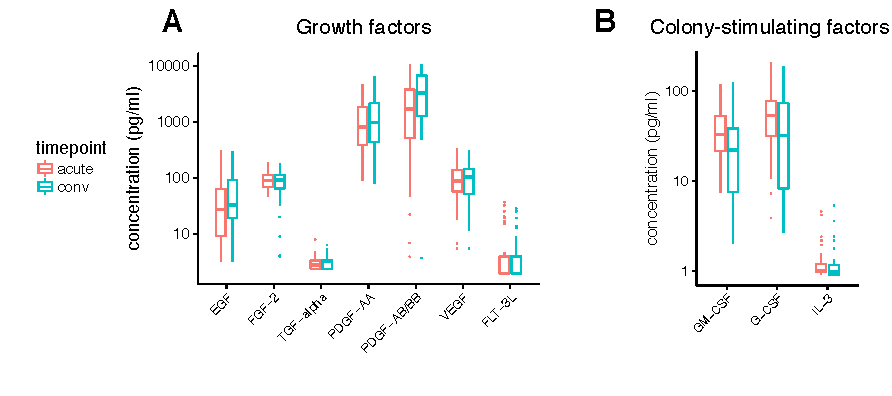
\includegraphics[width=0.8\textwidth]{chap6/fig_S10_nonsig_luminex}
  \fullwidthlabelcaption{fig:nonsig_luminex}{Differences in serum growth factor and colony-stimulating factor levels between the acute and convalescent timepoints}{
  \textbf{Differences in serum growth factor and colony-stimulating factor levels between the acute and convalescent timepoints}, as measured by multiplex ELISA (Luminex). None of the differences depicted here achieved statistical significance at FDR < 0.05 (Wilcoxon signed-rank test).
  }
\end{figure*}

\begin{figure*}[p]
  \centering
  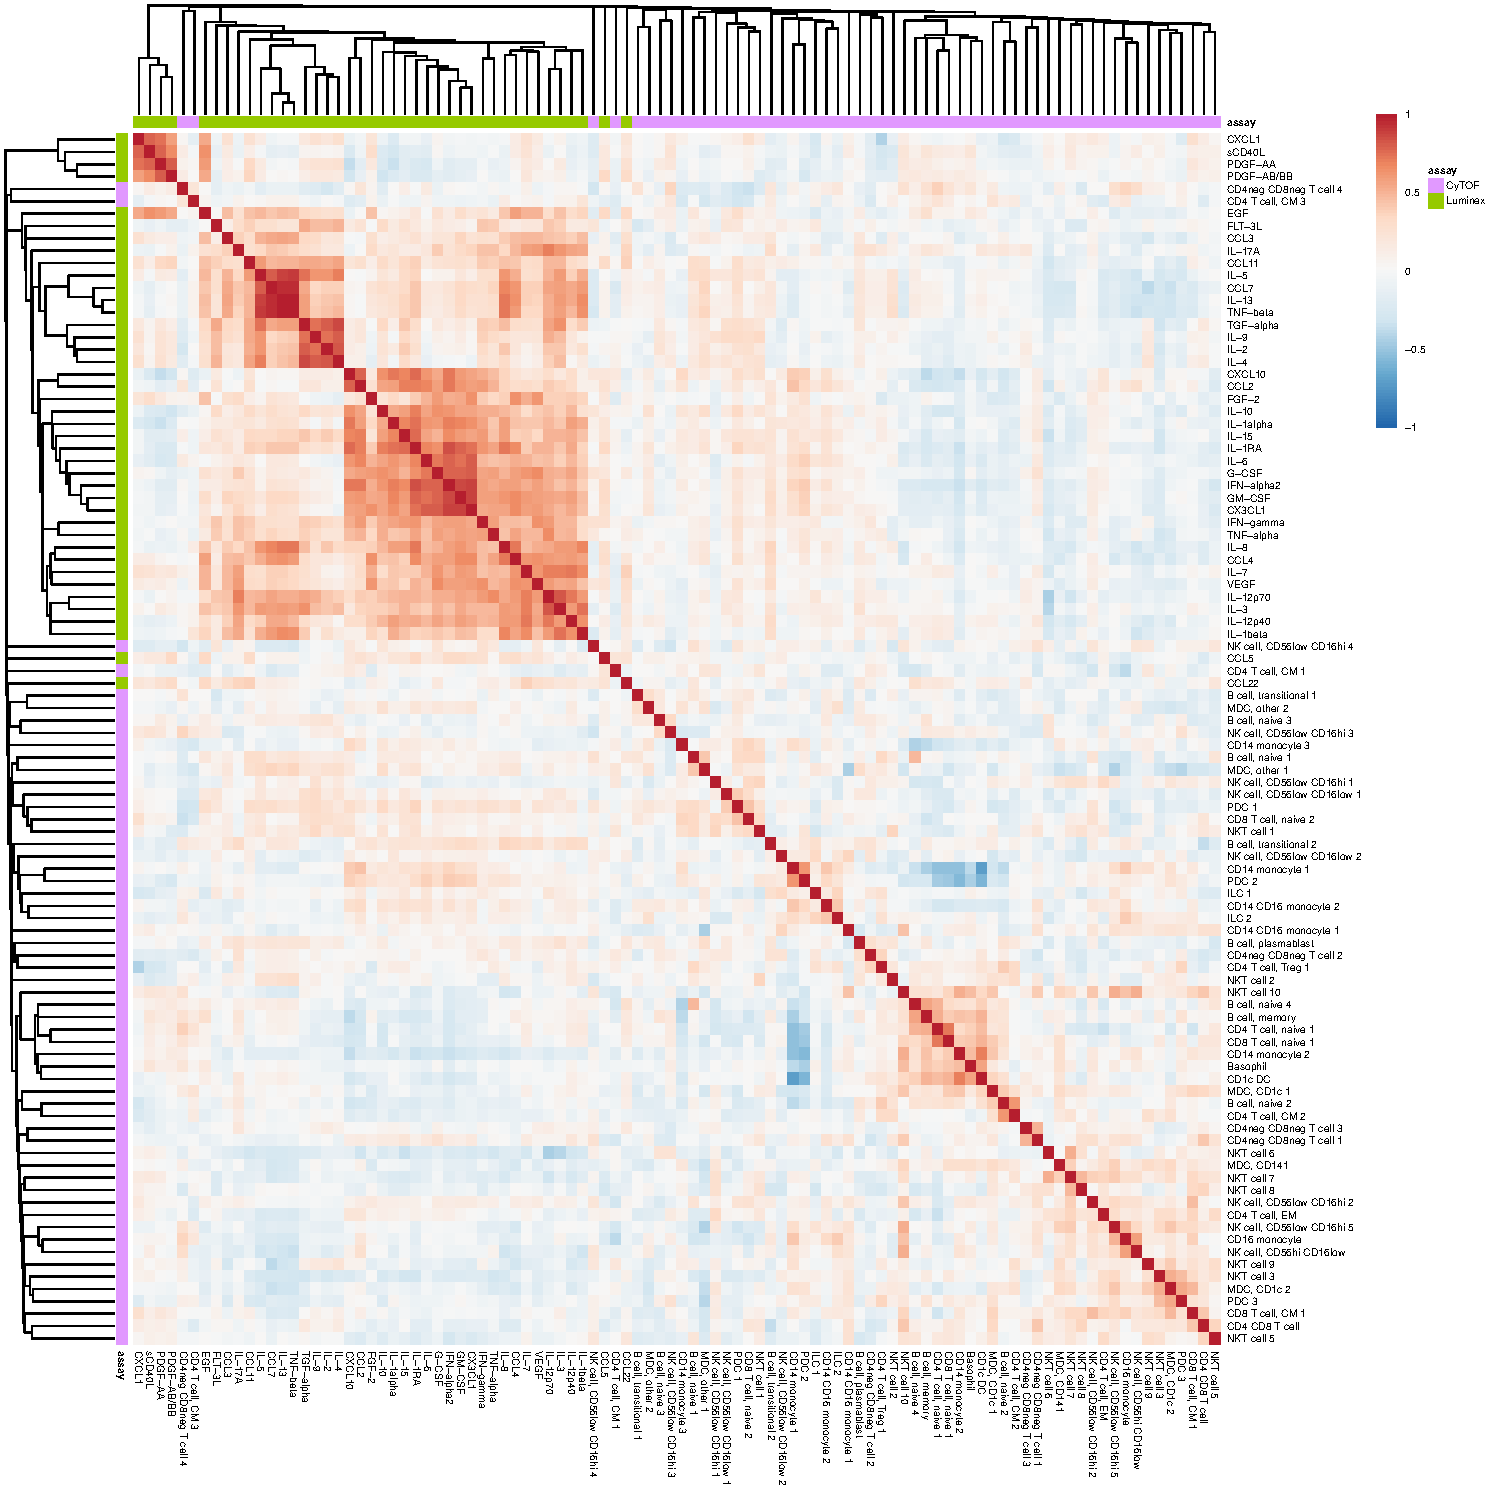
\includegraphics[width=\textwidth]{chap6/fig_S11_corrplot_luminex-cytof_all_both-times}
  \fullwidthlabelcaption{fig:corrplot_luminex_cytof_bothtimes}{Clustered heatmap of Pearson correlations between log-scaled serum cytokine concentration (Luminex) and log-scaled cell subphenotype frequencies (CyTOF) across the acute and convalescent timepoints}{
  \textbf{Clustered heatmap of Pearson correlations between log-scaled serum cytokine concentration (Luminex) and log-scaled cell subphenotype frequencies (CyTOF) \emph{across the acute and convalescent timepoints}}. The source of each variable (CyTOF vs. Luminex) is depicted by the pink-green annotation bar.
  }
\end{figure*}

\begin{figure*}[p]
  \centering
  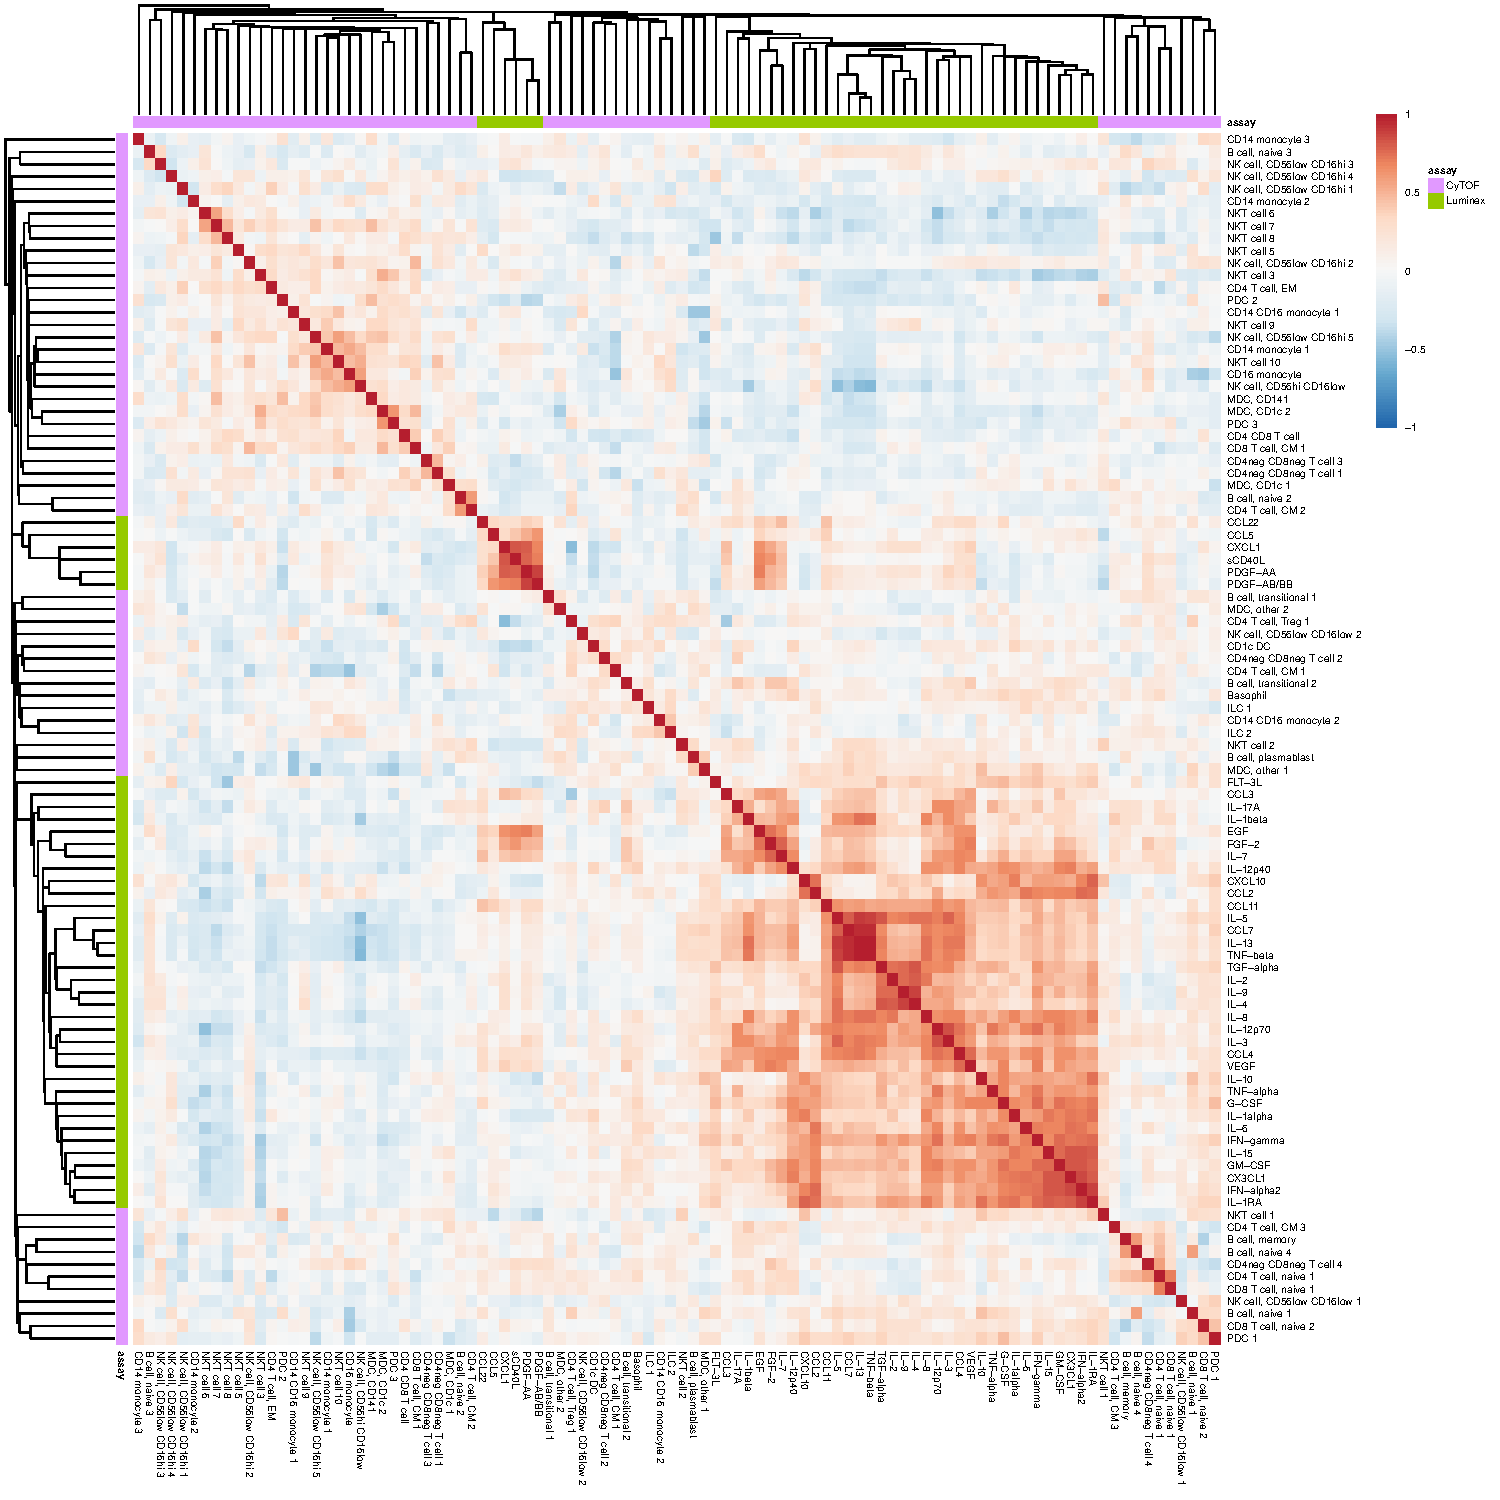
\includegraphics[width=\textwidth]{chap6/fig_S12_corrplot_luminex-cytof_all_acute}
  \fullwidthlabelcaption{fig:corrplot_luminex_cytof_acute}{Clustered heatmap of Pearson correlations between log-scaled serum cytokine concentration (Luminex) and log-scaled cell subphenotype frequencies (CyTOF) within the acute timepoint}{
  \textbf{Clustered heatmap of Pearson correlations between log-scaled serum cytokine concentration (Luminex) and log-scaled cell subphenotype frequencies (CyTOF) \emph{within the acute timepoint}}. The source of each variable (CyTOF vs. Luminex) is depicted by the pink-green annotation bar.
  }
\end{figure*}

\begin{figure*}[p]
  \centering
  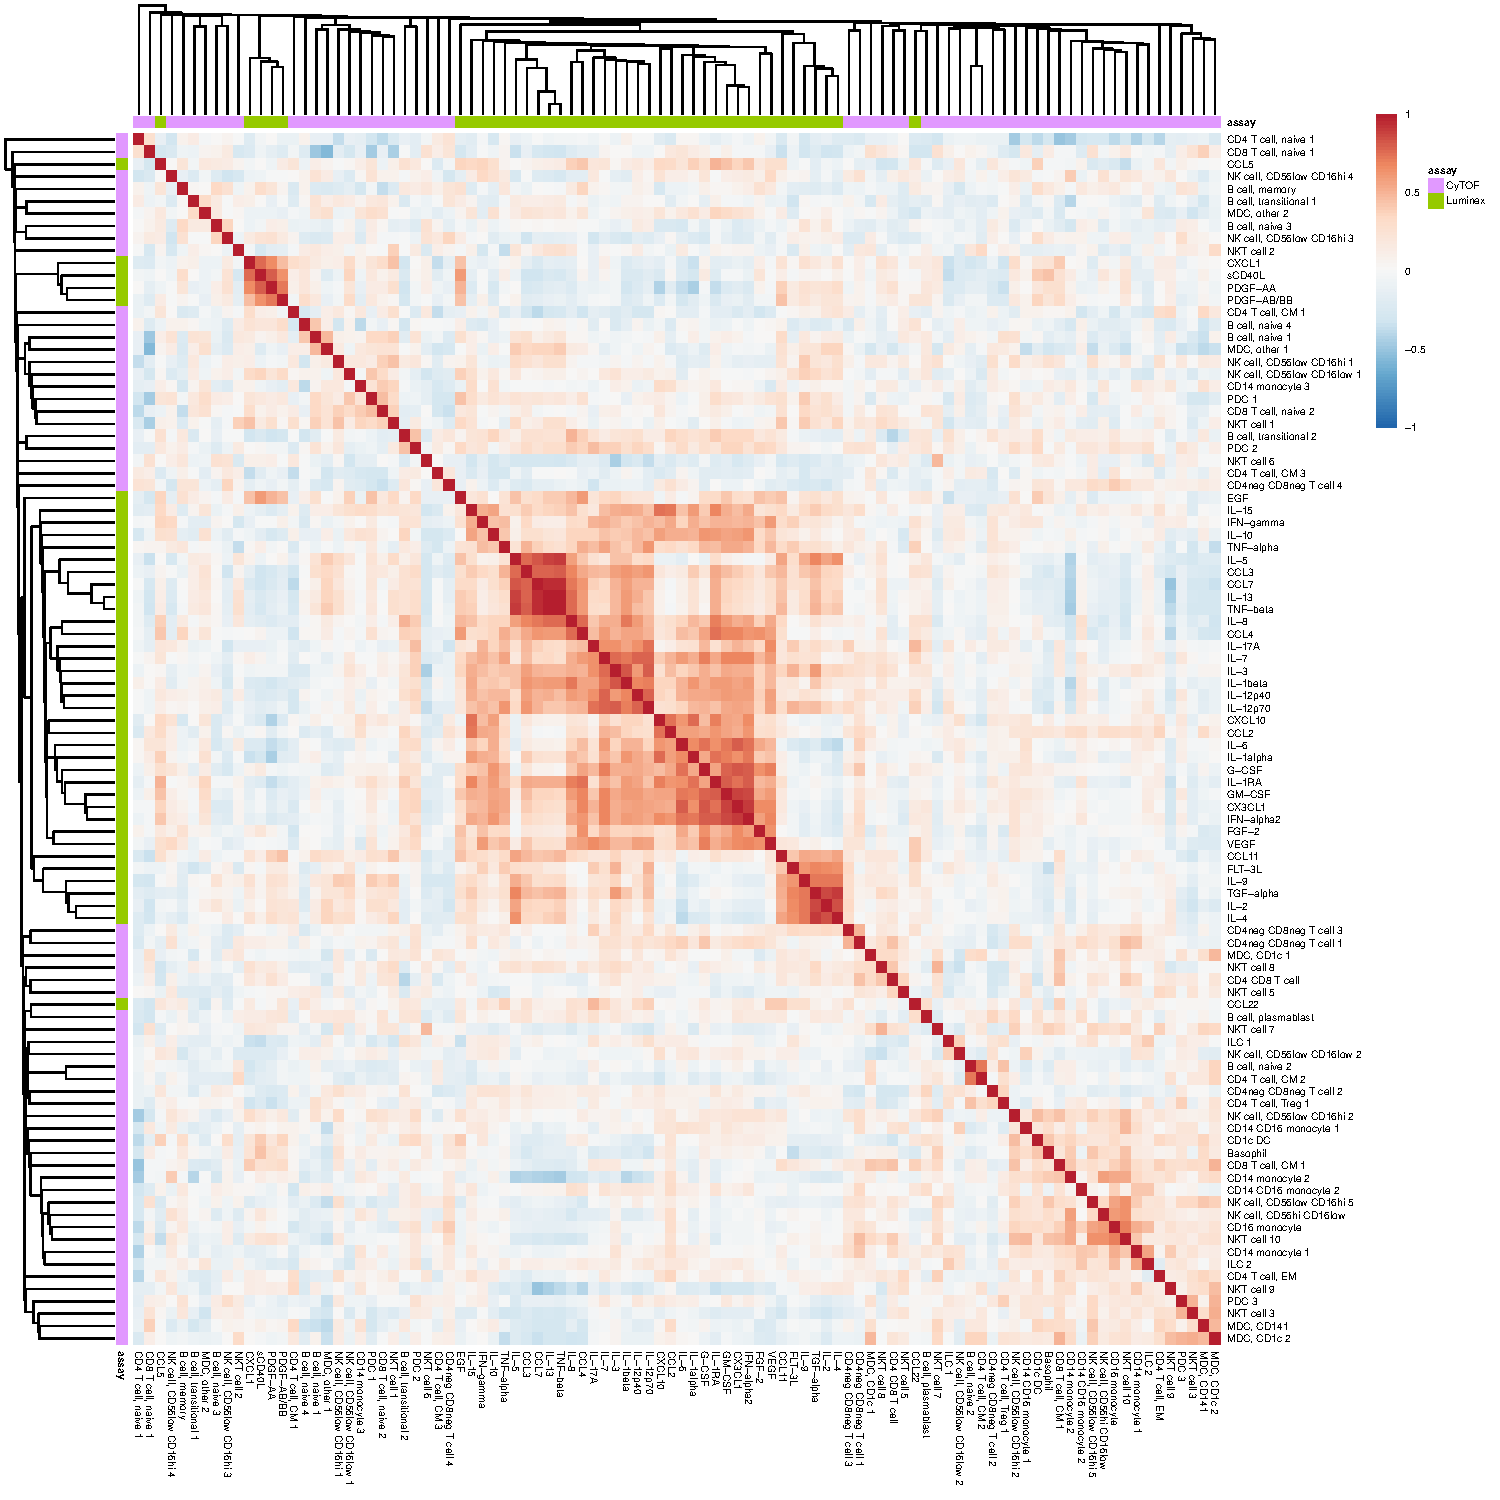
\includegraphics[width=\textwidth]{chap6/fig_S13_corrplot_luminex-cytof_all_conv}
  \fullwidthlabelcaption{fig:corrplot_luminex_cytof_conv}{Clustered heatmap of Pearson correlations between log-scaled serum cytokine concentration (Luminex) and log-scaled cell subphenotype frequencies (CyTOF) within the convalescent timepoint}{
  \textbf{Clustered heatmap of Pearson correlations between log-scaled serum cytokine concentration (Luminex) and log-scaled cell subphenotype frequencies (CyTOF) \emph{within the convalescent timepoint}}. The source of each variable (CyTOF vs. Luminex) is depicted by the pink-green annotation bar.
  }
\end{figure*}

\begin{figure*}[p]
  \centering
  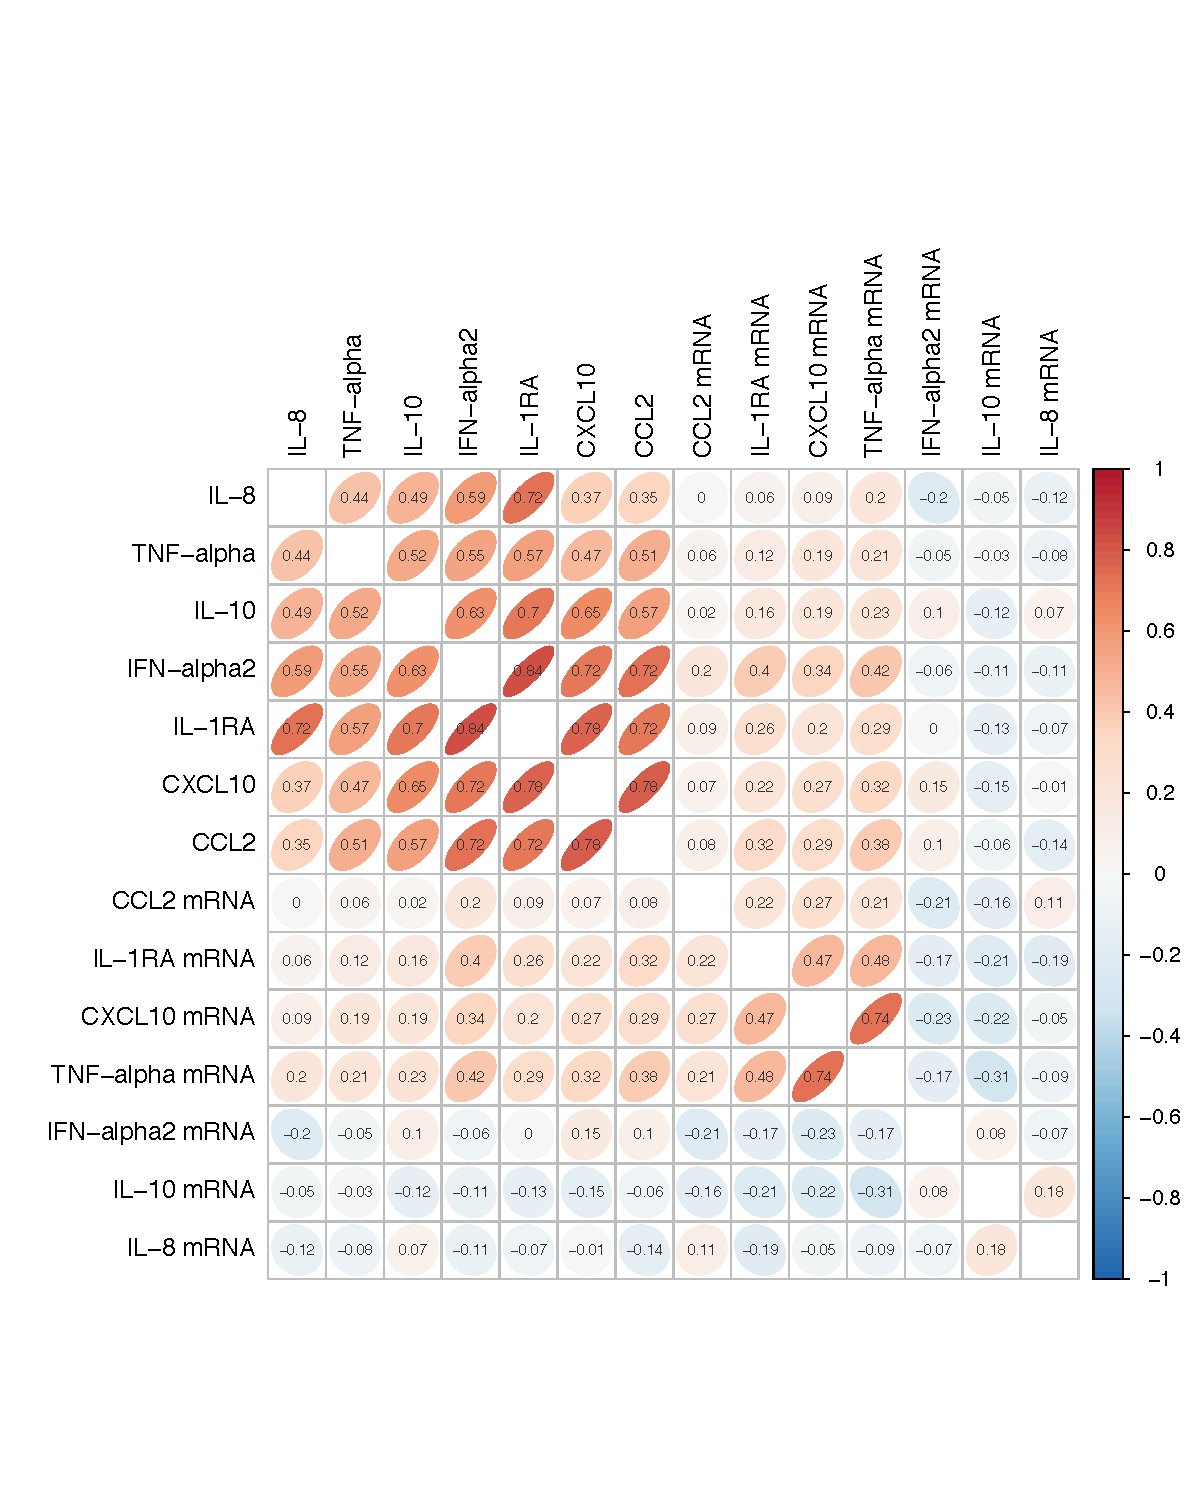
\includegraphics[width=\textwidth]{chap6/fig_S15_corrplot_luminex-mrna_cytokines_both}
  \fullwidthlabelcaption{fig:corrplot_luminex_mrna_both}{Pearson’s correlations between serum cytokine concentrations that were significantly different between timepoints and expression levels for corresponding genes}{
  \textbf{Pearson’s correlations between serum cytokine concentrations that were significantly different between acute and convalescent timepoints and expression levels (in FPKM) for corresponding genes.} Both values were log scaled before calculating Pearson’s~\emph{r}.
  }
\end{figure*}

\begin{figure*}[p]
  \centering
  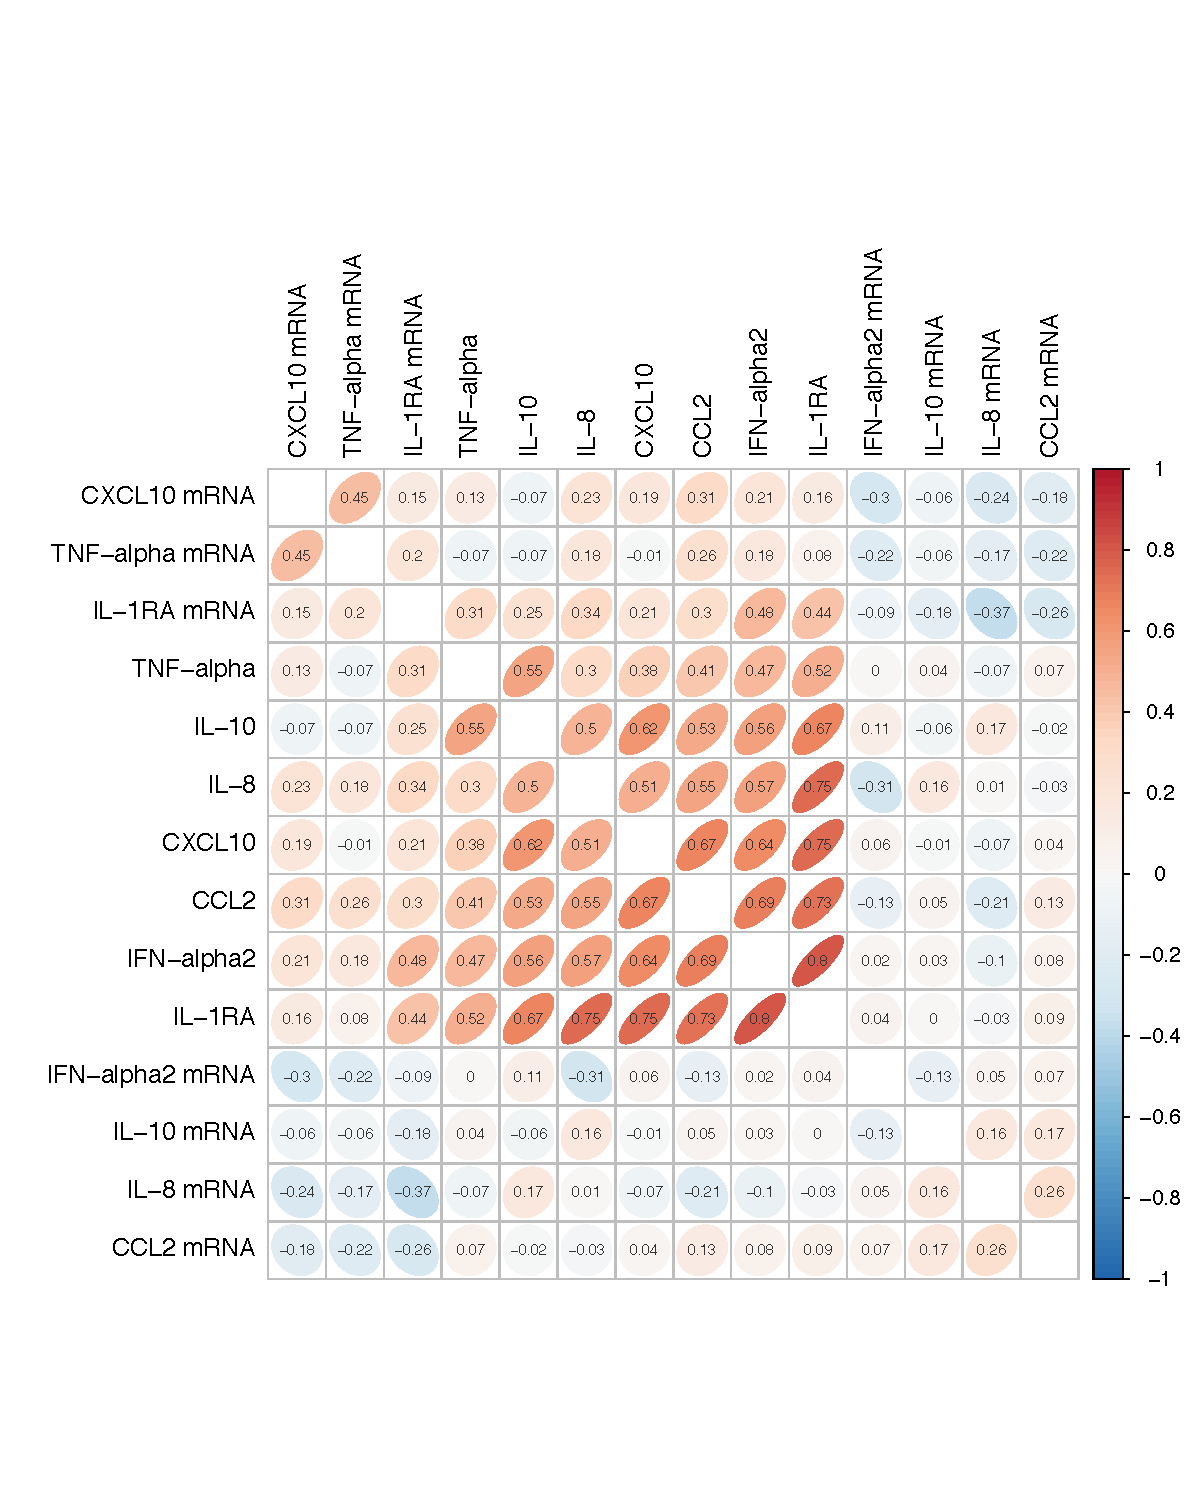
\includegraphics[width=\textwidth]{chap6/fig_S16_corrplot_luminex-mrna_cytokines_acute-minus-conv}
  \fullwidthlabelcaption{fig:corrplot_luminex_mrna_normacuteconv}{Pearson’s correlations between serum cytokine concentrations that were significantly different between timepoints and expression levels for corresponding genes, normalizing acute against convalescent}{
  \textbf{Pearson’s correlations between serum cytokine concentrations that were significantly different between acute and convalescent timepoints and expression levels (in FPKM) for corresponding genes, normalizing all values at the acute timepoint against convalescent values.} Normalized values were log scaled before calculating Pearson’s~\emph{r}.
  }
\end{figure*}

%%%%%
%
% Pathview plots, gene expression changes
%
%%%%%

\begin{sidewaysfigure}[hp]
  \centering
  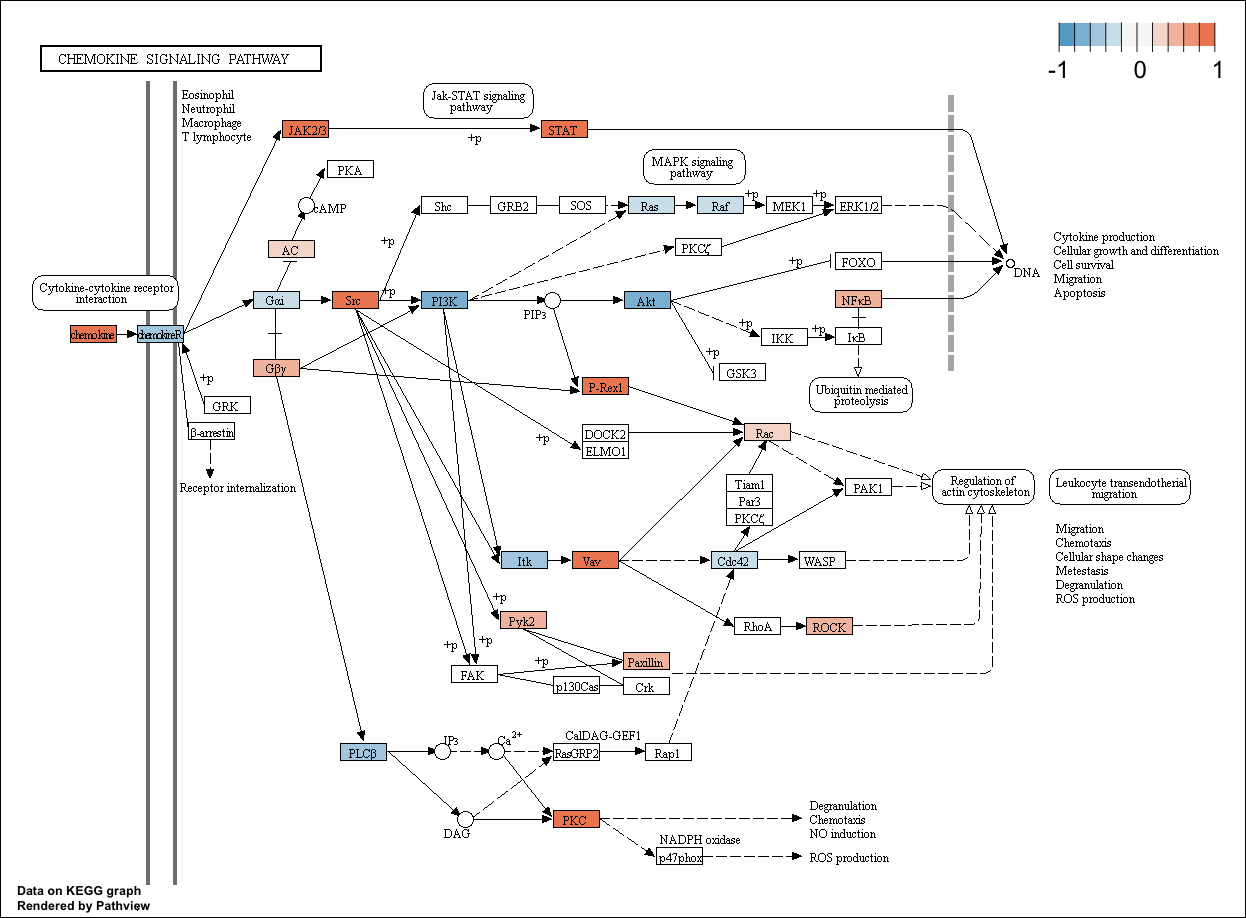
\includegraphics[width=\textwidth]{chap6/fig_S18_hsa04062.timepoint.log2fc.png}
  \fullwidthlabelcaption{fig:pathview_hsa04062}{Pathview plot of log\subs{2} fold change in expression of chemokine signaling pathway genes}{
  \textbf{Pathview plot of log\subs{2} fold change in gene expression between acute and convalescent timepoints for the chemokine signaling pathway}, using KEGG annotations (accession \href{http://www.genome.jp/dbget-bin/www\textunderscore bget?hsa04062}{hsa04062}). Positive values indicate upregulation during the acute phase of infection.
  }
\end{sidewaysfigure}

\begin{sidewaysfigure}[hp]
  \centering
  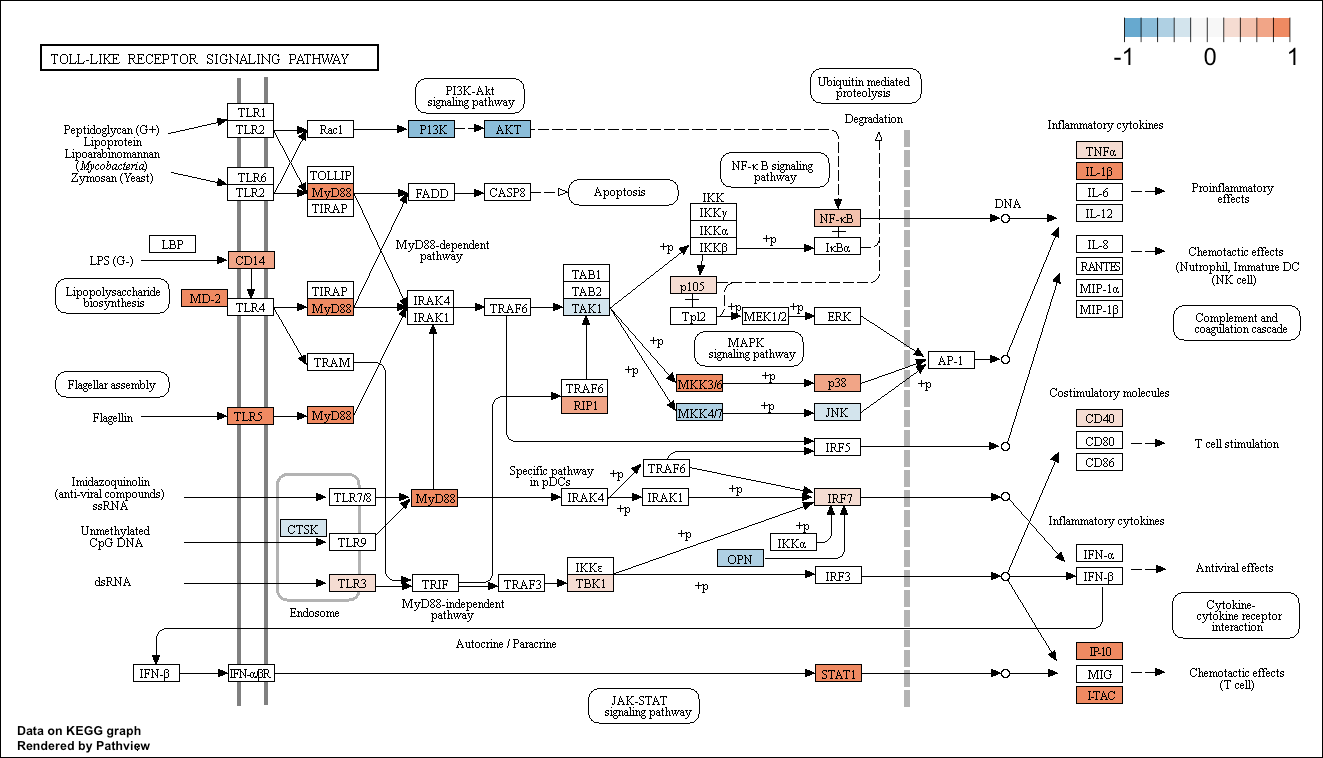
\includegraphics[width=\textwidth]{chap6/fig_S19_hsa04620.timepoint.log2fc.png}
  \fullwidthlabelcaption{fig:pathview_hsa04620}{Pathview plot of log\subs{2} fold change in expression of toll-like receptor pathway genes}{
  \textbf{Pathview plot of log\subs{2} fold change in gene expression between acute and convalescent timepoints for the toll-like receptor pathway}, using KEGG annotations (accession \href{http://www.genome.jp/dbget-bin/www\textunderscore bget?hsa04620}{hsa04620}). Positive values indicate upregulation during the acute phase of infection.
  }
\end{sidewaysfigure}

\begin{sidewaysfigure}[hp]
  \centering
  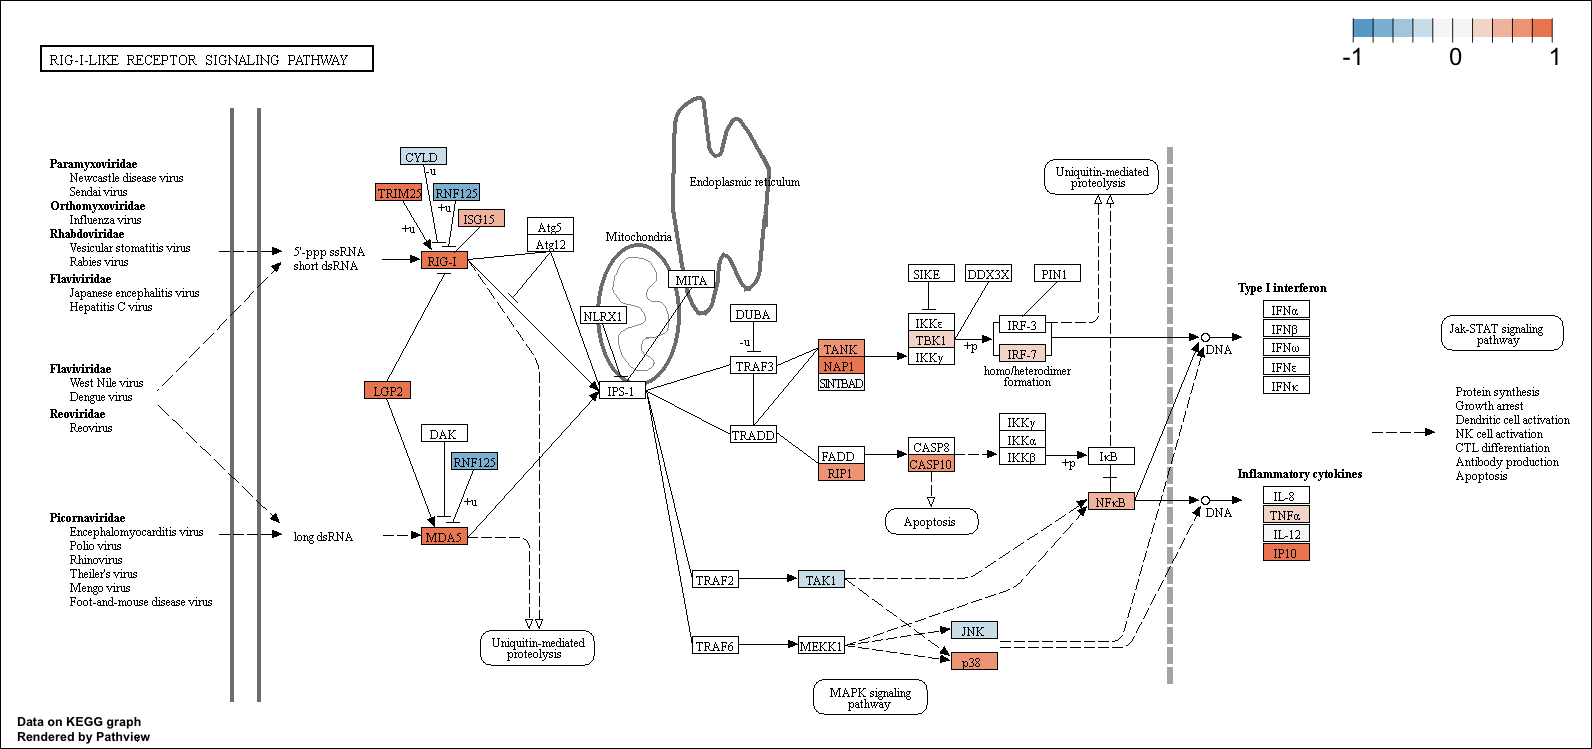
\includegraphics[width=\textwidth]{chap6/fig_S20_hsa04622.timepoint.log2fc.png}
  \fullwidthlabelcaption{fig:pathview_hsa04622}{Pathview plot of log\subs{2} fold change in expression of RIG-I-like receptor signaling pathway genes}{
  \textbf{Pathview plot of log\subs{2} fold change in gene expression between acute and convalescent timepoints for the RIG-I-like receptor signaling pathway}, using KEGG annotations (accession \href{http://www.genome.jp/dbget-bin/www\textunderscore bget?hsa04622}{hsa04622}). Positive values indicate upregulation during the acute phase of infection.
  }
\end{sidewaysfigure}

\begin{sidewaysfigure}[hp]
  \centering
  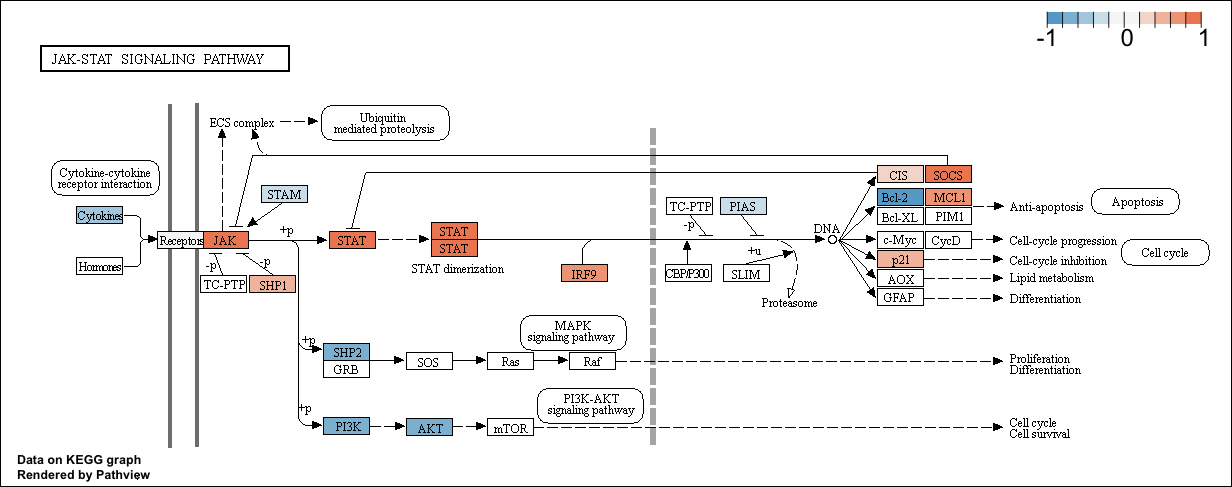
\includegraphics[width=\textwidth]{chap6/fig_S21_hsa04630.timepoint.log2fc.png}
  \fullwidthlabelcaption{fig:pathview_hsa04630}{Pathview plot of log\subs{2} fold change in expression of JAK-STAT signaling pathway genes}{
  \textbf{Pathview plot of log\subs{2} fold change in gene expression between acute and convalescent timepoints for the JAK-STAT signaling pathway}, using KEGG annotations (accession \href{http://www.genome.jp/dbget-bin/www\textunderscore bget?hsa04630}{hsa04630}). Positive values indicate upregulation during the acute phase of infection.
  }
\end{sidewaysfigure}

\begin{sidewaysfigure}[hp]
  \centering
  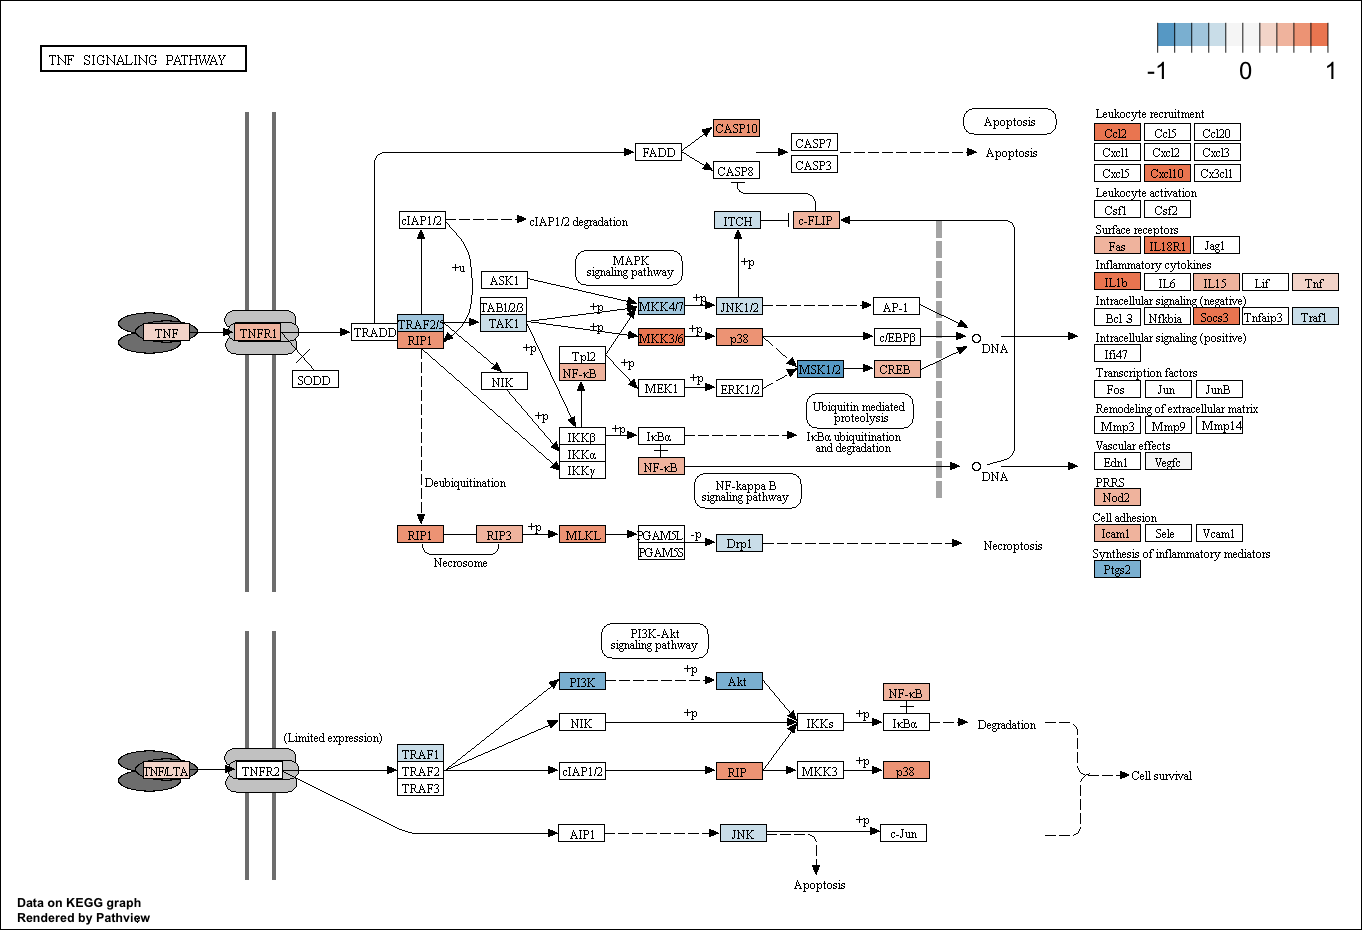
\includegraphics[width=\textwidth]{chap6/fig_S22_hsa04668.timepoint.log2fc.png}
  \fullwidthlabelcaption{fig:pathview_hsa04668}{Pathview plot of log\subs{2} fold change in expression of TNF signaling pathway genes}{
  \textbf{Pathview plot of log\subs{2} fold change in gene expression between acute and convalescent timepoints for the TNF signaling pathway}, using KEGG annotations (accession \href{http://www.genome.jp/dbget-bin/www\textunderscore bget?hsa04668}{hsa04668}). Positive values indicate upregulation during the acute phase of infection.
  }
\end{sidewaysfigure}

\begin{figure*}[hp]
  \centering
  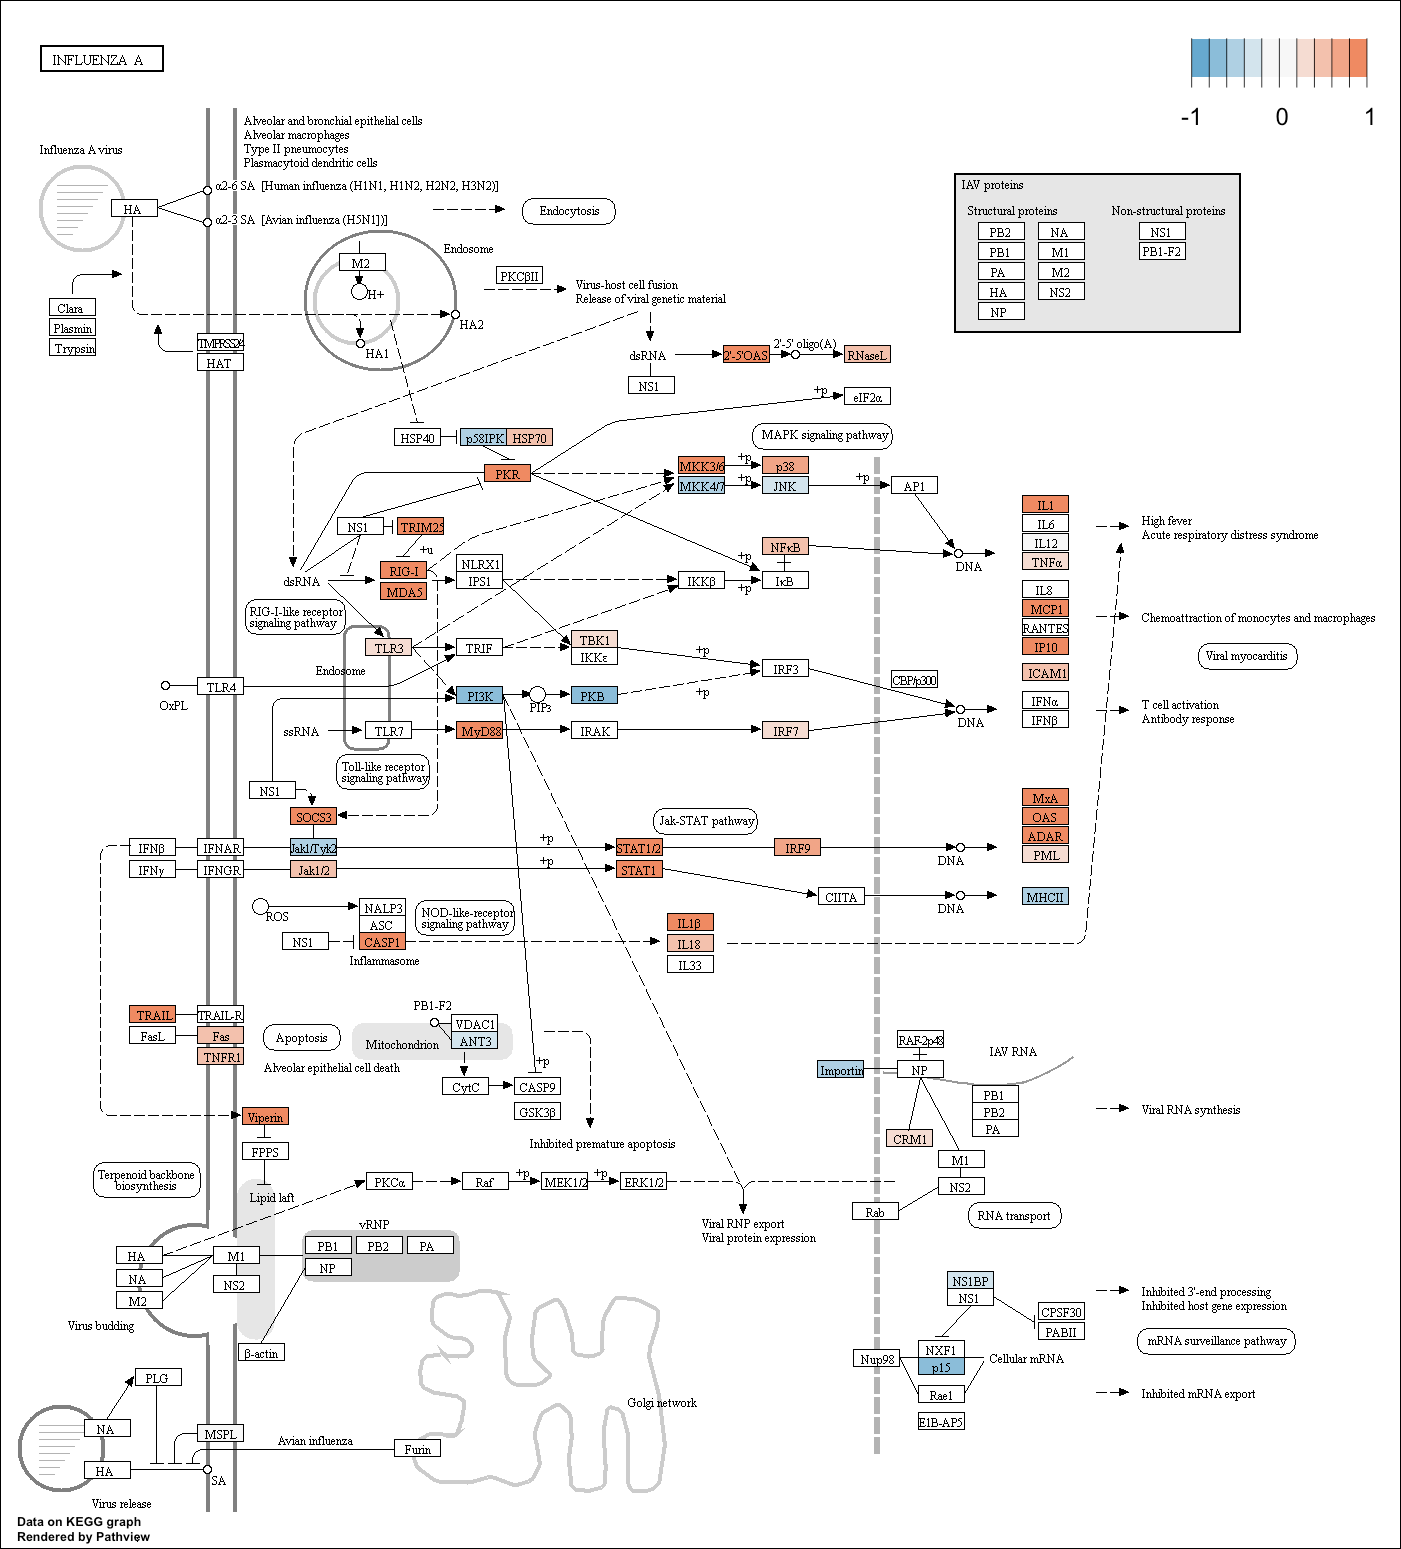
\includegraphics[width=\textwidth]{chap6/fig_S23_hsa05164.timepoint.log2fc.png}
  \fullwidthlabelcaption{fig:pathview_hsa05164}{Pathview plot of log\subs{2} fold change in expression of Influenza A pathway genes}{
  \textbf{Pathview plot of log\subs{2} fold change in gene expression between acute and convalescent timepoints for the Influenza A pathway}, using KEGG annotations (accession \href{http://www.genome.jp/dbget-bin/www\textunderscore bget?hsa05164}{hsa05164}). Positive values indicate upregulation during the acute phase of infection.
  }
\end{figure*}

%%%%%
%
% Less exciting network stuff
%
%%%%%

\begin{figure*}[hp]
  \centering
  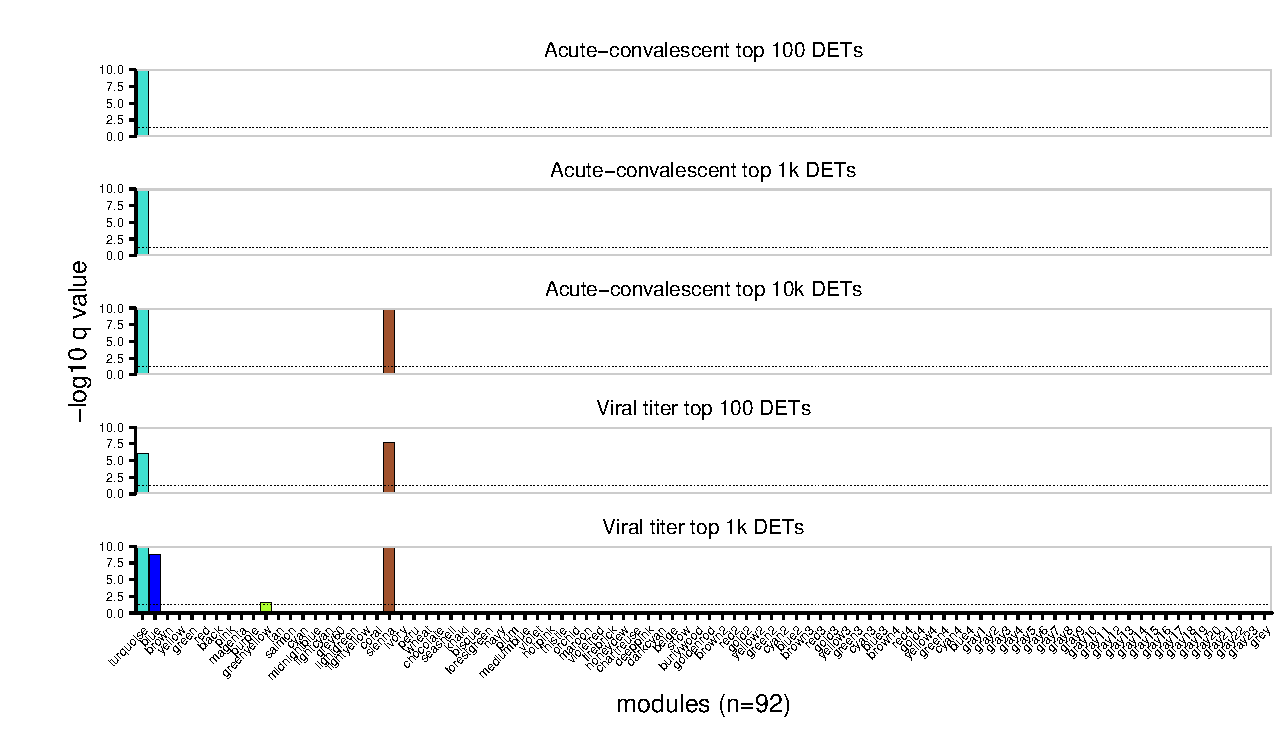
\includegraphics[width=\textwidth]{chap6/fig_S25_coexpp_net_25_modules_DET_overlaps_qvals}
  \fullwidthlabelcaption{fig:coem_det_overlap_qvals}{\emph{q} values for enrichment analyses of five DET signatures among the 92 coexpression modules}{
  \textbf{\emph{q} values (Benjamini-Hochberg adjusted \emph{P} values; Fisher’s exact test) for enrichment analyses of five differentially expressed transcript signatures among the 92 coexpression modules}. Coexpression modules were created using whole genome coexpression network analysis; see Figure \ref{fig:chik_TOM}. The horizontal dashed line corresponds to a  significance threshold of \emph{q} = 0.05.
  }
\end{figure*}

\begin{figure*}[hp]
  \centering
  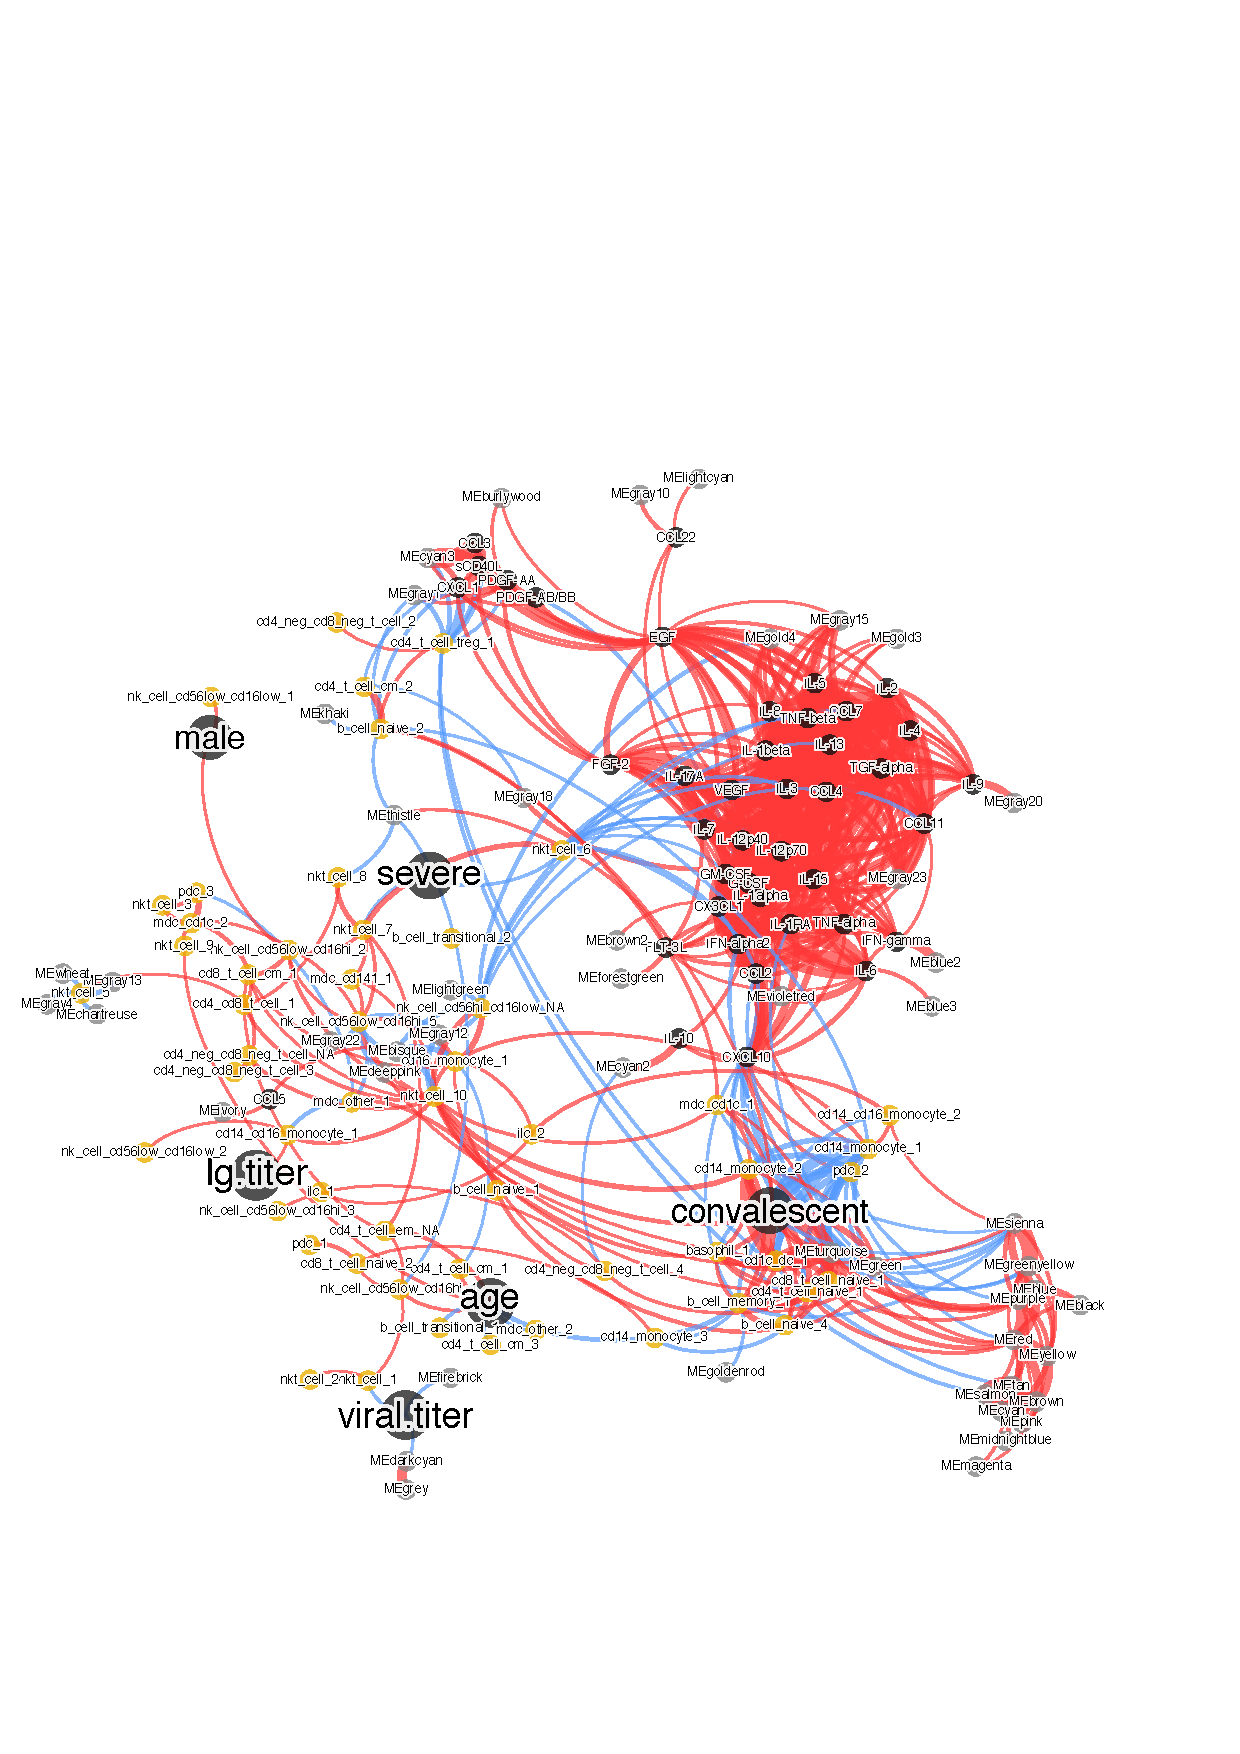
\includegraphics[width=\textwidth]{chap6/fig_S26_cytof-luminex-genemodules}
  \fullwidthlabelcaption{fig:multiscale_w_luminex}{Weighted multiscale interaction network including Luminex data}{
  \textbf{Weighted multiscale interaction network including Luminex data.} Edges represent all Pearson’s correlations between subpopulation frequencies (gold nodes), serum cytokine concentrations (small black nodes), coexpression modules (gray nodes), and clinical variables (large black nodes), filtered to correlations significant at \emph{P} < 0.001. Thickness is scaled to the magnitude of the correlation. The serum cytokines form a large interconnected component at top right that is not correlated with any of the clinical variables.
  }
\end{figure*}

% Restore the geometry of tufte-latex's big right margin
\restoregeometry
% Restore tufte-latex's fancy header/footer offsets
\tuftefancyhfoffset

\clearpage
\newpage

% Recalculate fancy header/footer after geometry change (otherwise page numbers are misplaced)
%\fancyhfoffset[E,O]{0pt}
